\documentclass[reqno]{amsart}
\newtheorem{theorem}{Theorem}[section]
\newtheorem{lemma}[theorem]{Lemma}
\newtheorem{proposition}[theorem]{Proposition}
\theoremstyle{definition}
\newtheorem{definition}[theorem]{Definition}
\newtheorem{example}[theorem]{Example}
\newtheorem{xca}[theorem]{Exercise}
\usepackage[a4paper, left=3.25cm, right=3.25cm, top=3.5cm, bottom=3.5cm]{geometry}
\theoremstyle{remark}
\usepackage{caption}
\newtheorem{remark}[theorem]{Remark}
\numberwithin{equation}{section}
\newcommand{\be}{\begin{eqnarray}}
\newcommand{\en}{\end{eqnarray}}
\newcommand{\nn}{\nonumber}
\newcommand{\bmf}{\boldsymbol}
\newcommand{\mr}{\mathrm}
\newcommand{\abs}[1]{\lvert#1\rvert}
% \newcommand{\firstauthor}[1]{#1$^{\dagger}$}
\newcommand{\corrauthor}[1]{#1$^{*}$}
\usepackage{graphicx}
\usepackage{subfigure}
\usepackage{amsmath}
\usepackage{epstopdf}
\usepackage{dsfont}
\usepackage{varioref}
\usepackage{hyperref}
\usepackage{cleveref}
\usepackage{color}
\usepackage{mathrsfs,amsfonts}
\usepackage{tikz}
\usepackage{graphicx}
\usetikzlibrary{patterns}
\usepackage{circuitikz}
\usepackage{tkz-base,tkz-euclide}
\usepackage{cite}

\newcommand{\blankbox}[2]{%
  \parbox{\columnwidth}{\centering
    \setlength{\fboxsep}{0pt}%
    \fbox{\raisebox{0pt}[#2]{\hspace{#1}}}%
  }%
}

\graphicspath{{figures/}}

\begin{document}
\title{Finite volume element method for Landau-Lifshitz equation}
%    Information for first author
\author{Yunjie Gong}
%    Address of record for the research reported here
\address{School of Mathematical Sciences, Soochow University, Suzhou 215006, China}
% %    Current address
% \curraddr{School of Mathematical Sciences, Soochow University, Suzhou 215006, China}
\email{gyj1564763342@163.com}
%    \thanks will become a 1st page footnote.
%\thanks{The first author was supported in part by NSF Grant \#000000.}


\author{\corrauthor{Rui Du}}
\address{School of Mathematical Sciences, Soochow University, Suzhou 215006, China}
\email{durui@suda.edu.cn}
%    Information for second author
\author{\corrauthor{Panchi Li}}
\address{Department of Mathematics, The University of Hong Kong, Hong Kong, China}
\address{Materials Innovation Institute for Life Sciences and Energy (MILES), HKU-SIRI, Shenzhen, China.}
\email{lipch@hku.hk}
%\thanks{Support information for the second author.}
%    General info

% \subjclass[2000]{Primary 54C40, 14E20; Secondary 46E25, 20C20}

% \date{January 1, 2023 and, in revised form, June 22, 2001.}

%\dedicatory{This paper is dedicated to our advisors.}
\thanks{$^{*}$ Corresponding authors.}


\begin{abstract}
The Landau-Lifshitz equation describes the dynamics of magnetization in ferromagnetic materials. Due to the essential nonlinearity and nonconvex constraint, it is typically solved numerically.
In this paper,
we developed a finite volume element method (FVEM) with the Gauss-Seidel projection method (GSPM) for the micromagnetics simulations.
We give the error estimate for FVEM in space and depict the discretized energy dissipation.
Owing to the application of the GSPM,
the nonlinear vector system is decoupled and the computational complexity is comparable to that of implicitly solving the scalar heat equation,
which accelerates the real simulations significantly.
We present several numerical experiments to verify the theoretical analysis.
Furthermore,
we study the blow-up solution and efficiently simulate the 2D magnetic textures using the proposed method.
\end{abstract}

\subjclass{65N12; 65M60}
\keywords{Finite volume element method; Landau-Lifshitz equation; micromagnetics simulations; phenomenon of blow-up}


\maketitle


\section{Introduction}
In micromagnetics, the fundamental quantity of interest is the magnetization,
a three-dimensional vector field with a constant magnitude at the lattice point when the system is below the Curie temperature.
Under various external controls, the system exhibits interesting dynamic behaviors and would reach equilibrium guided by the Landau-Lifshitz~(LL) equation~\cite{Landau}.
When the system reaches static equilibrium, many magnetic textures, such as the domain wall, vortex and skyrmion, can be generated, which relates to local stationary points of the magnetic free energy.
The LL equation consists of the gyromagnetic and damping terms and is weakly nonlinear, and
due to the constant length of magnetization in a point-wise sense, the energy functional becomes non-convex.
These pose challenges to the theoretical analysis and numerical studies of the LL equation.

In past decades,
the mathematical theory and numerical methods for the LL equation have garnered significant attention \cite{Kruz,Maekawa,Shinjo,Melcher,Zhou}.
The existence and uniqueness of weak solutions have been established in \cite{Alouges,Carbou1,Guo}.
Alouges and Soyeur established the existence of the global weak solution in the three-dimensional case \cite{Alouges}.
Guo and Hong demonstrated the global existence of solutions and uncovered new connections between harmonic maps and the solutions of the LL equation \cite{Guo}.
On the other hand, numerous researchers are devoted to developing the numerical methods for the LL equation.
Based on the finite difference method (FDM),
Milton and Donahue \cite{Miltat} proposed efficient approaches grounded in field-based and energy-based formulations for micromagnetics simulations.
Fuwa et al. \cite{Fuwa} proposed an implicit nonlinear scheme and provided its unique solvability.
Recently,
Chen et al. \cite{chen} developed a second-order semi-implicit projection method for micromagnetics simulations in which the spatial step size is of the same order as the temporal step size.
Meanwhile, numerical approaches based on the finite element method (FEM) have been continuously developed. Bartels and Prohl \cite{Bartels} proposed a fully implicit nonlinear scheme and demonstrated its unconditional stability.
Soon afterward,
Alouges et al. \cite{Alouges1,Alouges2,Alouges3} developed a fully discrete linearized $\theta$-scheme and provided the corresponding stability condition.
Gao \cite{Gao} proposed a linearized backward Euler method and established optimal error estimates in both $L^2$ and $H^1$ norms.
Besides, An \cite{an} proved the optimal error estimates for the linearized Crank-Nicolson Galerkin method. Among these approaches, either a nonlinear system or a linearized system with variable coefficients must be resolved due to the nonlinearity of the equation. To accelerate simulations' efficiency, a series of Guass-Seidel projection methods (GSPMs) have been developed in the past decades~\cite{GSPM2001JCP,Li,li2024enhanced}, in which only linear equations with constant coefficients need to be solved.

Our work is inspired by the finite volume element method (FVEM) for nonlinear parabolic equations \cite{chen1,chen2}.
The FVEM, also known as the generalized difference method, is different from the FEM and FDM.
Its basic idea is to approximate the discrete fluxes needed in the classical finite volume method (FVM) by replacing the finite element approximation of the solution for PDEs \cite{cai1}.
%This implies that the discretization focuses more on the local characteristics of the solution,
%rather than the equations themselves, by selecting appropriate finite element spaces.
%The theory and basic framework of the FVEM have been developed in the past few decades (see, e.g.\cite{cai1,cai2,lin1,lin2,rose,hack,mishev,lironghua,chat1}).
Similar to the FEM, the FVEM exhibits a capability of handling complex boundary conditions and irregular geometries. Moreover, it usually has a simpler solver structure and is conducive to implementing advanced techniques with low computational costs.
In this paper, we develop a novel approach for the LL equation that combines the FVEM in space and the GSPM in time.
For the spatial error estimate, we construct a linear auxiliary problem with variable coefficients and prove the approximation error of the FVEM.
In a specific setup, the auxiliary problem becomes a linearized implicit scheme of the LL equation, allowing us to estimate the approximation error for the original problem. Thereafter, the discrete energy dissipation is naturally obtained. Since the GSPM is adopted for time evolutions, the convergence analysis of the temporal error cannot be given. We conduct several numerical experiments to verify the convergence rates in both time and space. Furthermore, using the proposed method, we study the blow-up solution of the LL equation and static magnetic textures of 2D ferromagnetic films with the Dirichlet boundary condition. Numerical results showcase that our method provides a promising approach to simulating complex systems with high efficiency.

The rest of this paper is organized as follows.
In \Cref{Sec2:Basic Model and numerical methods}, we introduce the basis model and the FVEM.
In \Cref{Sec3:Some auxiliary lemmas and error analysis for FVE method}, we give the error estimate and depict the discretized energy dissipation.
The numerical approach is detailed and numerical tests are conducted as in \Cref{sec4: Temporal discretization and numerical experiments}.
Conclusions are drawn in \Cref{sec5:Conclusions}.


\section{Mathematical Model and numerical methods \label{Sec2:Basic Model and numerical methods}}
\subsection{The LL equation}
The fundamental LL equation reads as
\begin{equation*}
\partial_t\bmf{M}
=
-\mu_0\gamma\bmf{M} \times \mathcal{H}
- \frac{ \mu_0\gamma \alpha } {{M}_s} \bmf{M} \times (\bmf{M} \times \mathcal{H}),
\label{LL1}
\end{equation*}
where $M_s = |\bmf{M}|$ is the saturation magnetization,
$\gamma$ is the gyromagnetic ratio,
$\alpha$ is the damping parameter,
$\mu_0$ is the magnetic permeability of vacuum,
and $\mathcal{H}$ is the effective field given by the variation calculation $\mathcal{H} = -(1/\mu_0)\delta\mathcal{F}/\delta\bmf{M}$ of the magnetic free energy
\begin{equation*}
\mathcal{F}[\bmf{M}]
=
\int_{\Omega}\frac{A}{M_s^2}|\nabla \bmf{M}|^2 \,\mr{d}\bmf{x}
+
\int_{\Omega}\Phi\left(\frac{\bmf{M}}{M_s}\right)\,\mr{d}\bmf{x}
-
\mu_0\int_{\Omega}\bmf{H}_{\mr{e}}\cdot\bmf{M}\,\mr{d}\bmf{x}
+
\frac{\mu_0}{2}\int_{\Omega}\bmf{H}_{\mr{s}} \cdot \bmf{M}\,\mr{d}\bmf{x}.
\label{LL2}
\end{equation*}
In the energy functional, $\Omega$ denotes the volume occupied by the ferromagnetic body, $A$ is the exchange constant,
$\Phi\left(\frac{\bmf{M}}{M_s}\right)$ is a smooth function that defines the anisotropy, and
$\bmf{H}_{\mr{e}}$ is the external magnetic field.
And in the last term,
$\bmf{H}_{\mr{s}}$ denotes the stray field and it is simplified to $\bmf{H}_{\mr{s}} \cdot \bmf{M} = {M}_3^2$ since ultra-thin films are considered in this work. Let the uniaxial anisotropy be along with $\bmf{e}_1 = (1, 0, 0)^T$,
and the effective field is given by
\begin{equation*}
\mathcal{H}
=
-\frac{\delta \mathcal{F}}{\delta \bmf{M}}
=
\frac{2 A}{M_s^2}\Delta \bmf{M}
-
\frac{2 K_{u}}{M_s^2}(M_2\bmf{e_2}+M_3\bmf{e_3})
-
\mu_0 M_3 \bmf{e}_3
+
\mu_0 \bmf{H}_{\mr{e}},
\end{equation*}
where $\bmf{e}_2=(0,1,0)^T$, $\bmf{e}_3=(0,0,1)^T$.
Define $\bmf{m}=M_s \bmf{M}$, $\bmf{H}_{\mr{s}} = M_s \bmf{h}_{\mr{s}}$ and $\bmf{H}_{\mr{e}}=M_s \bmf{h}_{\mr{e}}$,
and we get $\mathcal{F} = (\mu_0 M_s^2)F$ with
\begin{equation*}
F[\bmf{m}]
=
\frac{\epsilon}{2} \int_{\Omega}|\nabla \bmf{m}|^2 \,\mr{d}\bmf{x}
+
\frac{q}{2} \int_{\Omega}({m}_2^2+{m}_3^2) \,\mr{d}\bmf{x}
-
\int_{\Omega}\bmf{h}_{\mr{e}}\cdot\bmf{m} \,\mr{d}\bmf{x}
+
\frac{1}{2}\int_{\Omega}{m}_3^2 \,\mr{d}\bmf{x},
% \label{LL3}
\end{equation*}
in which we use the spatial rescaling $\bmf{x}\rightarrow L \bmf{x}$ and
\begin{equation*}
    \epsilon=\frac{2 A}{\mu_0 M_s^2 L^2},\quad q=\frac{2 K_{u}}{\mu_0 M_s^2}.
\end{equation*}
Furthermore, applying the time rescaling $ t\rightarrow (\mu_0 \gamma M_s)^{-1}t$ yields the dimensionless LL equation
\begin{equation}
\partial_t\bmf{m}
=
-
\bmf{m} \times {\bmf{h}}
-
\alpha \bmf{m} \times (\bmf{m} \times {\bmf{h}}),
\label{LL4}
\end{equation}
where
\begin{equation*}
\bmf{h} = \epsilon\Delta \bmf{m}-q(m_2\bmf{e_2}+m_3\bmf{e_3})-m_3 \bmf{e_3}+ \bmf{h}_{\mr{e}}.
\end{equation*}
To illustrate the main ideas of the numerical approach, we consider the simplified equation
\begin{equation*}
  \partial_t\bmf{m}
  =
  -
  \bmf{m} \times \Delta\bmf{m}
  -
  \alpha \bmf{m} \times (\bmf{m} \times \Delta\bmf{m}).
\end{equation*}
Due to the non-convex constraint $|\bmf{m}| = 1$,
this equation can be rewritten into
\begin{equation}
  \partial_t\bmf{m}
  -
  \alpha\Delta\bmf{m}
  +
  \bmf{m} \times \Delta\bmf{m}
  =
  \alpha |\nabla\bmf{m}|^2\bmf{m}.
  \label{equ:simplicity-LL-dimensionless}
\end{equation}
For the well-posedness, we adopt the initial condition and the Dirichlet boundary condition
\begin{gather}
    \bmf{m}(\bmf{x}, 0) = \bmf{m}_0(\bmf{x} ),\quad x\in \Omega\label{initial-condition}\\
    \bmf{m}(\bmf{x} ) = \bmf{g}(\bmf{x} ), \quad x\in\partial\Omega,\label{boundary}
\end{gather}
in which $|\bmf{m}_{0}| = |\bmf{g}| = 1$ holds in a point-wise sense.

\subsection{FVEM approximation}
We begin by introducing some notations that will be used throughout this paper.
The standard notation of Sobolev spaces $W^{s,p}(\Omega)$ ($1\leq p\leq\infty$) consists of functions that have generalized derivatives of order $s$ in $L^p(\Omega)$ that equips the norm
\begin{equation*}
\|m\|_{W^{s,p}}
=
\left( \int_{\Omega}\sum_{|\alpha|\leq s}|D^{\alpha}m|^{p} \, \mr{d}x \right)^{\frac{1}{p}}
\end{equation*}
with the standard modification for $p=\infty$. We then use
\( \bmf{L}^p \) and \( \bmf{W}^{k,r} \) to denote the vector Sobolev space $ (L^p(\Omega))^3 $ and $(W^{k,r}(\Omega))^3$, respectively.
In particular, we write \( \bmf{H}^k :=\bmf{W}^{k,2} \), and particularly define
$$\bmf{X} = L^{\infty}([0, T]; \bmf{H}^{2}(\Omega)) \cap L^2([0, T]; \bmf{H}^3(\Omega)).$$
% Furthermore, the partial derivative $\frac{\mr{d}}{\mr{dt}}$ will be denoted as $\mr{d}_t$.

\begin{figure}[htbp]
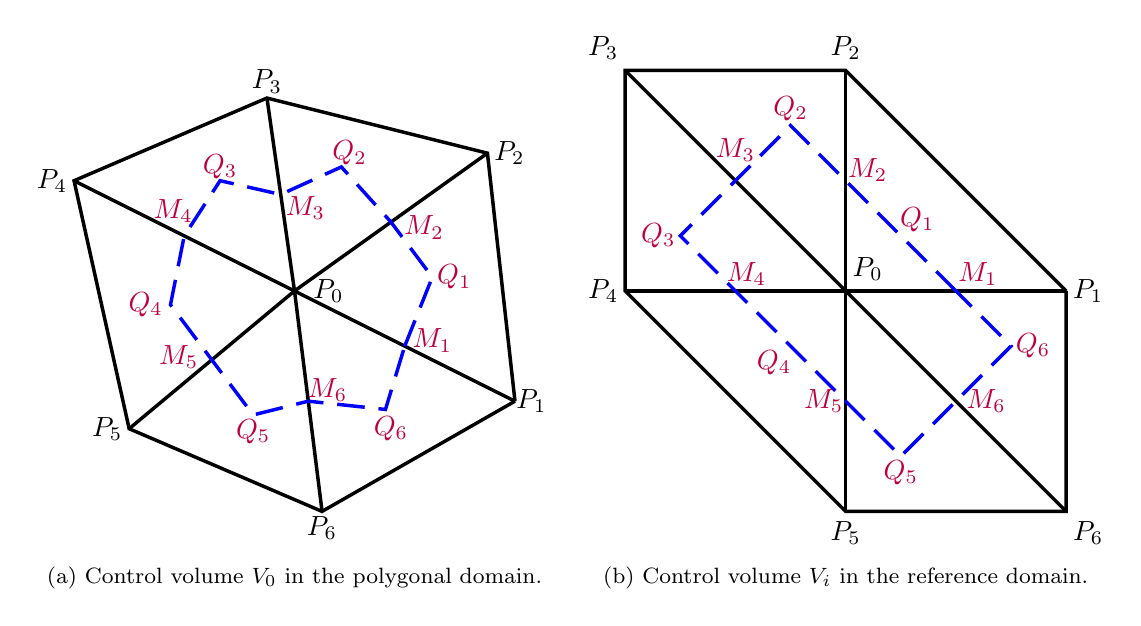
\begin{tikzpicture}[>=latex,scale=0.7]
\begin{scope}
		 \draw[line width = 1.25pt] (0,0)node[right=0.1cm]{$P_0$} --  (4,-2);node%[left=0.1cm]{$P_1$};
		 \draw[line width = 1.25pt] (0,0) -- (3.5,2.5);%node[right=0.1cm]{$P_2$};
		 \draw[line width = 1.25pt] (0,0) -- (-0.5,3.5);%node[above=0.1cm]{$P_3$};
         \draw[line width = 1.25pt] (0,0) -- (-4,2);%node[left=0.1cm]{$P_4$};
         \draw[line width = 1.25pt] (0,0) -- (-3,-2.5);%node[left=0.1cm]{$P_5$};
         \draw[line width = 1.25pt](0,0) -- (0.5,-4);%node[below=0.1cm]{$P_6$};
         %%%%%%%%%%%%%%%%%%%%%%%%%%%%%%%%%%%%%%%%%%%%%%%%%%%
        \draw[line width = 1.25pt] (4,-2) to (3.5,2.5) to (-0.5,3.5) to(-4,2) to (-3,-2.5) to (0.5,-4) to (4,-2);
%%%%%%%%%%%%%%%%%%%%%%%%%%%%%%%%%%%%%%%%%%%%%%%%%%%
         \draw[dash pattern = on 10pt off 5pt, line width = 1.25pt, color = blue]
         (2,-1)%node[right=0.1cm]{$M_1$}
         to (2.5,0.25)%node[right=0.1cm]{$Q_1$}
         to (1.75,1.25)%node[below=0.1cm]{$M_2$}
         to(0.85,2.25)%node[above=0.1cm]{$Q_2$}
         to (-0.25,1.75)%node[above=0.1cm,right = 0.1cm]{$M_3$}
         to (-1.35,2)%node[above=0.1cm]{$Q_3$}
         to (-2,1)%node[left=0.1cm]{$M_4$}
         to (-2.25,-0.25)%node[left=0.1cm]{$Q_4$}
         to (-1.5,-1.25)%node[below=0.05cm]{$M_5$}
         to (-0.75,-2.25)%node[below=0.1cm]{$Q_5$}
         to (0.25,-2)%node[below=0.1cm]{$M_6$}
         to (1.65,-2.15)%node[below=0.1cm]{$Q_6$}
         to (2,-1);
         %%%%%%%%%%%%%%%%%%%%%%%%%%%%%%
         %\node at (0,0) {\TeX};
         %\node [<options>] (<name>) at(<coordinate>){<node contents>};
         \node at (4.3,-2){$P_1$};
         \node at (3.9,2.5){$P_2$};
         \node at (-0.5,3.8){$P_3$};
         \node at (-4.4,2){$P_4$};
         \node at (-3.4,-2.5){$P_5$};
         \node at (0.5,-4.3){$P_6$};
         \node[text=purple] at (2.5,-0.9){$M_1$};
         \node[text=purple] at (2.35,1.15){$M_2$};
         \node[text=purple] at (0.2,1.5){$M_3$};
         \node[text=purple] at (-2.2,1.45){$M_4$};
         \node[text=purple] at (-2.1,-1.2){$M_5$};
         \node[text=purple] at (0.6,-1.8){$M_6$};
         \node[text=purple] at (2.9,0.25){$Q_1$};
         \node[text=purple] at (1,2.5){$Q_2$};
         \node[text=purple] at (-1.35,2.25){$Q_3$};
         \node[text=purple] at (-2.7,-0.25){$Q_4$};
         \node[text=purple] at (-0.75,-2.55){$Q_5$};
         \node[text=purple] at (1.75,-2.5){$Q_6$};
          \node at (0,-5.2){\footnotesize (a) Control volume $V_0$ in the polygonal domain.};
          \end{scope}
%%%%%%%%%%%%%%%%%%%%%%%%%%%%%%
\begin{scope}[xshift = 10cm]
		 \draw[line width = 1.25pt] (0,0)%node[above=0.2cm,left=0.1cm]{$P_0$}
		 --  (4,0);%node[right=0.1cm]{$P_1$};
		 \draw[line width = 1.25pt] (0,0) -- (0,4);%node[right=0.1cm]{$P_2$};
		 \draw[line width = 1.25pt] (0,0) -- (-4,4);%node[left=0.1cm]{$P_3$};
         \draw[line width = 1.25pt] (0,0) -- (-4,0);%node[left=0.1cm]{$P_4$};
         \draw[line width = 1.25pt] (0,0) -- (0,-4);%node[left=0.1cm]{$P_5$};
         \draw[line width = 1.25pt] (0,0) -- (4,-4);%node[right=0.1cm]{$P_6$};
         %%%%%%%%%%%%%%%%%%%%%%%%%%%%%%%%%%%%%%%%%%%%%%%%%%%%%%%%%
        \draw[line width = 1.25pt] (4,0) to (0,4) to (-4,4) to(-4,0) to (0,-4) to (4,-4) to (4,0);
         %%%%%%%%%%%%%%%%%%%%%%%%%%%%%%%%%%%%%%%%%%%%%%%%%%%
         \draw[dash pattern = on 10pt off 5pt, line width = 1.25pt, color = blue]
         (2,0)%node[right=0.1cm]{$M_1$}
         to (1,1)%node[right=0.1cm]{$Q_1$}
         to (0,2)%node[below=0.1cm]{$M_2$}
         to (-1,3)%node[above=0.1cm]{$Q_2$}
         to (-2,2)%node[above=0.1cm,right = 0.1cm]{$M_3$}
         to (-3,1)%node[above=0.1cm]{$Q_3$}
         to (-2,0)%node[left=0.1cm]{$M_4$}
         to (-1,-1)%node[left=0.1cm]{$Q_4$}
         to (0,-2)%node[below=0.05cm]{$M_5$}
         to (1,-3)%node[below=0.1cm]{$Q_5$}
         to (2,-2)%node[below=0.1cm]{$M_6$}
         to (3,-1) %node[below=0.1cm]{$Q_6$}
         to (2,0);
         %%%%%%%%%%%%%%%%%%%%%%%%%%%%%%
         %\node at (0,0) {\TeX};
         %\node [<options>] (<name>) at(<coordinate>){<node contents>};
         \node at (0.4,0.4){$P_0$};
         \node at (4.4,0){$P_1$};
         \node at (0,4.4){$P_2$};
         \node at (-4.4,4.4){$P_3$};
         \node at (-4.4,0){$P_4$};
         \node at (0,-4.4){$P_5$};
         \node at (4.4,-4.4){$P_6$};
         \node[text=purple] at (2.4,0.3){$M_1$};
         \node[text=purple] at (0.4,2.2){$M_2$};
         \node[text=purple] at (-2,2.55){$M_3$};
         \node[text=purple] at (-1.8,0.3){$M_4$};
         \node[text=purple] at (-0.4,-2){$M_5$};
         \node[text=purple] at (2.55,-2) {$M_6$};
         \node[text=purple] at (1.3,1.3){$Q_1$};
         \node[text=purple] at (-1,3.3){$Q_2$};
         \node[text=purple] at (-3.4,1){$Q_3$};
         \node[text=purple] at (-1.3,-1.3){$Q_4$};
         \node[text=purple] at (1,-3.3){$Q_5$};
         \node[text=purple] at (3.4,-1){$Q_6$};
         \node at (0,-5.2){\footnotesize (b) Control volume $V_i$ in the reference domain.};
	 \end{scope}	
  \end{tikzpicture}
 \caption{The control volume $V_0$ centered at $P_0$ in the polygonal domain and a reference domain.}
\label{Fig1}
\end{figure}

For a polygonal domain $\Omega$,
we consider the quasi-uniform regular triangulation $T_h$ consisting of closed triangle elements $K$ such that $\bar{\Omega}=\cup_{K\in T_h}K$.
$\mathcal{N}_h$ denotes the set of all nodes with $N = |\mathcal{N}_h|$, and then define $\mathcal{N}_h^{0} = \mathcal{N}_h\cap\Omega$.
In~\Cref{Fig1}(a), for the FVEM we represent the control volume of the node $P_0$ with
the polygon $ M_1 Q_1 M_2 Q_2 M_3 Q_3 M_4 Q_4 M_5 Q_5 M_6 Q_6 $,
where $M_i$ and $Q_i$ $(i = 1, \cdots, 6)$ are the points on edges and in the interior of elements, respectively.
For clarity, we introduce the control volume $V_i$ in the reference triangle as in \Cref{Fig1}(b).
The control volume $V_i$ in the polygonal domain and the corresponding control volume in the reference triangle can be obtained through an affine transformation.
For any arbitrary point $ P_i \in \mathcal{N}_h$, control volumes $V_i$ associated with each node $P_i$ form the dual mesh $T_h^*$ in the polygonal region.

Let $h$ denote the maximum diameter of all elements in $T_h$.
We assume that the dual mesh $T_h^*$ is quasi-uniformly regular, i.e., there exists a positive constant $C$ such that
\begin{equation*}
C^{-1}h^2 \leq \mr{mean}(V_i) \leq Ch^2, \quad \forall\; V_i\in T_h^*.
\end{equation*}
Denote $S_h$ the approximation space on $T_h$ as
\begin{equation*}
S_h
=
\{v\in C(\bar{\Omega}):\ v|_K\ \text{is piecewise linear for all} \, K\in T_h\},
\end{equation*}
and the dual volume element space $S_h^*$ on $T_h^*$ is
\begin{equation*}
S^*_h
=
\{v\in L^2(\Omega):\ v|_{V_i}\ \text{is piecewise constant for all} \ V_i\in T_h^*\}.
\end{equation*}
Let $\phi_i(\bmf{x})$ be the standard nodal basis function associated with the node $\bmf{x}_i$. We have $S_h=\mathrm{span}\{\phi_i(\bmf{x}):\bmf{x}_i\in\mathcal{N}_h^0\}$ and
$S_h^*=\mathrm{span}\{\phi^*_i(\bmf{x}):\bmf{x}_i\in\mathcal{N}_h^0\}$,
where $\phi_i^*(\bmf{x})$ is the characteristic function of $V_i$.

For the LL equation, we use $\bmf{S}_h$ and $\bmf{S}_h^*$ denote $(S_h)^3$ and $(S_h^*)^3$,
respectively. Then, define the interpolation operator $I_h:\bmf{H}_0^1\cap \bmf{H}^2\rightarrow \bmf{S}_h$ such that
\begin{equation*}
    I_h \bmf{v}
    =
    \sum_{\bmf{x}_i\in\mathcal{N}_h^0}\bmf{v}(\bmf{x}_i)\phi_i(\bmf{x}).
\end{equation*}
Meanwhile, for any $\bmf{v}_h\in \bmf{S}_h$, we define another interpolation operator $I_h^*:\bmf{S}_h\rightarrow \bmf{S}_h^*$,
such that
$$I_h^*\bmf{v}_h=\sum_{\bmf{x}_i\in\mathcal{N}_h^0}\bmf{v}_h(\bmf{x}_i)\phi_i^*(\bmf{x}).$$

For the numerical analysis, we assume that within finite time the LL equation \eqref{equ:simplicity-LL-dimensionless}-\eqref{boundary} has a unique local weak solution $\bmf{m}$ satisfying the regularity condition:
\begin{equation}
   \|\bmf{m}\|_{L^{\infty}(0,T;\bmf{H}^{3})}
   \! + \!
    \|\partial_t \bmf{m}\|_{L^2(0,T;\bmf{H}^2)}
   \! + \!
    \|\partial_t \bmf{m}\|_{L^{\infty}(0,T;\bmf{H}^1)}
   \! + \!
    \|\partial_{tt} \bmf{m} \|_{L^2(0,T;\bmf{L}^2)}
    \! \leq \!
    C.
    \label{regularity-condition}
\end{equation}
This is important because the solution may blow up with a smooth initial condition. Hence the
theoretical analysis in this work is not applicable to scenarios near the blow-up phenomena.
On the other hand, the following bound of the numerical solution is also required
\begin{equation*}
        \|\nabla \bmf{m}_h\|_{\bmf{L}^{\infty}} \leq C.
    % \label{working_set}
\end{equation*}

The FVEM approximation starts from
integrating \eqref{equ:simplicity-LL-dimensionless} over an control volume $V_i$ with the application of the Green's formula,
\begin{equation}
  \int_{V_i} \partial_t\bmf{m}_h \,\mr{d}x \mr{d}y
  -
  \int_{\partial V_i} \alpha \nabla \bmf{m}_h \cdot\bmf{n} \,\mr{d}S
  +
  \int_{\partial V_i} \bmf{m}_h \times (\nabla \bmf{m}_h \cdot\bmf{n}) \,\mr{d}S
  =
  \int_{V_i} \alpha |\nabla \bmf{m}_h|^2 \bmf{m}_h \,\mr{d}x\mr{d}y.
  \label{equ:simplicity-semi-discretized}
\end{equation}
Multiplying both sides of \eqref{equ:simplicity-semi-discretized} by $\bmf{v}_h(\bmf{x}_i)$ and taking the sum of all terms $\bmf{x}_i \in \mathcal{N}_h$ yields the discrete scheme for \eqref{equ:simplicity-LL-dimensionless}:
Find $\bmf{m}_h \in \bmf{S}_h$,
such that for all $\bmf{v}_h \in \bmf{S}_h$,
\begin{equation}
\left\{
\begin{aligned}
&(\partial_t\bmf{m}_h, I_h^*\bmf{v}_h)
 +
 \mathcal{A}_h(\bmf{m}_h;\bmf{m}_h,I_h^*\bmf{v}_h)
 =
 \alpha(|\nabla\bmf{m}_h|^2\bmf{m}_h,I_h^*\bmf{v}_h), \\
&\bmf{m}_h(0) = I_h \bmf{m}_0, \\
&\bmf{m}_h(t)|_{\partial\Omega} = \bmf{0},
\end{aligned}
\label{equ:LL-semi-discretized1}
\right.
\end{equation}
where $\mathcal{A}_h(\bmf{m}_h;\bmf{m}_h,I_h^*\bmf{v}_h)
    =
    a_h(\bmf{m}_h,I_h^*\bmf{v}_h)
    +
    b_h(\bmf{m}_h;\bmf{m}_h,I_h^*\bmf{v}_h)$ with
\begin{equation*}
 a_h(\bmf{m}_h,I_h^*\bmf{v}_h)
 =
 - \sum_{\bmf{x}_i\in\mathcal{N}_h}\!\int_{\partial V_i}\alpha\cdot\nabla \bmf{m}_h\cdot\bmf{n}\cdot I_h^*\bmf{v}_h \,\mr{d}S
 =
 - \sum_{\bmf{x}_i\in\mathcal{N}_h}\bmf{v}_h(\bmf{x}_i)\int_{\partial
V_i}\!\alpha \cdot\nabla \bmf{m}_h\cdot\bmf{n}\,\mr{d}S,
\end{equation*}
\begin{equation*}
 b_h(\bmf{m}_h;\bmf{m}_h,I_h^*\bmf{v}_h)
 \!=
 \!\!\!\sum_{\bmf{x}_i\in\mathcal{N}_h}\!\!\int_{\partial V_i}\!\!\!(\bmf{m}_h \! \times \! (\nabla \bmf{m}_h \cdot\bmf{n})) \cdot I_h^*\bmf{v}_h\,\mr{d}S\!
 =
 \!\!\!\sum_{\bmf{x}_i\in\mathcal{N}_h}\!\!\!\bmf{v}_h(\bmf{x}_i)\!\!\!\int_{\partial V_i}\!\!\!\bmf{m}_h \!\times\! (\nabla \bmf{m}_h \cdot\bmf{n}) \,\mr{d}S.
\end{equation*}
To prove the error estimate for FVEM in space and the discretized energy law, here we define $|||\bmf{m}_h|||_{0} = (\bmf{m}_h, I_h^*\bmf{m}_h)$ in $\bmf{S}_h$. It is easy to verify that there exist two positive constants $C_*, C^*$ independent of $h$ such that
\begin{equation*}
 C_*\|\bmf{m}_h\|_{\bmf{L}^2}\leq |||\bmf{m}_h|||_{0}\leq C^*\|\bmf{m}_h\|_{\bmf{L}^2},\quad
\forall \bmf{m}_h\in \bmf{S}_h.
\end{equation*}

Before the formal error analysis is given, we declare some inequalities. When the 2D space is considered,
there exists a constant $C$ such that for all $\bmf{v}\in \bmf{H}^2$,
the following inequalities hold:
\begin{eqnarray}\label{Sobolev-inequality}
\begin{aligned}
&\|\bmf{v}\|_{\bmf{L}^r}
\leq
C \|\bmf{v}\|_{\bmf{H}^1} \quad (2 \leq r \leq 6), \\
&\|\bmf{v}\|_{\bmf{L}^4}
\leq
C \|\bmf{v}\|_{\bmf{H}^1}^{\frac{1}{2}}\|\bmf{v}\|_{\bmf{L}^2}^{\frac{1}{2}},\\
&\|\bmf{v}\|_{\bmf{L}^{\infty}}
\leq
C (\|\bmf{v}\|_{\bmf{L}^2}^2 + \|\Delta \bmf{v}\|_{\bmf{L}^2}^2)^{\frac{1}{2}},\\
&\|\nabla \bmf{v}\|_{\bmf{L}^{\infty}}
\leq
C \|\nabla \bmf{v}\|_{\bmf{L}^2}^{\frac{1}{2}}
(\|\nabla \bmf{v}\|_{\bmf{L}^2}^2 + \|\Delta \bmf{v}\|_{\bmf{L}^2}^2 + \|\nabla \Delta \bmf{v}\|_{\bmf{L}^2}^2)^{\frac{1}{4}},\\
&\|\nabla\bmf{v}\|_{\bmf{L}^4}
\leq
C \|\nabla\bmf{v}\|_{\bmf{L}^2}^{\frac{1}{2}}
( \|\nabla\bmf{v}\|_{\bmf{L}^2}^{2} + \|\Delta \bmf{v}\|_{\bmf{L}^2}^{2})^{\frac{1}{4}},\\
&\|\Delta\bmf{v}\|_{\bmf{L}^4}
\leq
C \|\Delta\bmf{v}\|_{\bmf{L}^2}^{\frac{1}{2}}
( \|\Delta\bmf{v}\|_{\bmf{L}^2}^{2} + \|\nabla\Delta\bmf{v}\|_{\bmf{L}^2}^{2})^{\frac{1}{4}}.
\end{aligned}
\end{eqnarray}
In the sequel, we will use a uniform constant $C$ to denote all the controllable constants that are independent of spatial and temporal discretization parameters for simplicity of notation.


\section{Auxiliary lemmas and error estimates\label{Sec3:Some auxiliary lemmas and error analysis for FVE method}}

\subsection{An auxiliary problem}
We first define the auxiliary problem as follows:
Given a function $ \bmf{\Phi} \in \bmf{X}$, find $\tilde{\bmf{m}}$ such that
\begin{equation}
    \left\{\begin{aligned}
    &\partial_t\tilde{\bmf{m}}
    -
    \alpha \Delta\tilde{\bmf{m}}
    +
    \bmf{\Phi} \times \Delta \tilde{\bmf{m}}
    +
    \nabla\bmf{\Phi} \times \nabla \tilde{\bmf{m}}
    =
    \alpha |\nabla\bmf{\Phi}|^2 \tilde{\bmf{m}}, \\
    &\tilde{\bmf{m}} (x,y,0)
    =
    \tilde{\bmf{m}}_0, \\
    &\tilde{\bmf{m}}|_{\partial\Omega}
    =
    \bmf{0}.
    \end{aligned}\right.
    \label{equ:LL-auxiliary-problem}
\end{equation}
Let $\bmf{\Phi} = \tilde{\bmf{m}}$, and it becomes the LL equation. For any given $\bmf{\Phi}$, we compute the approximation error of the FVEM for this auxiliary problem. Then, we apply the fixed-point iteration and get the error estimate for the LL equation.
\begin{lemma}
    Given $ \bmf{\Phi} \in \bmf{X}$, there exists a positive constant $C$ such that
\begin{equation*}
        \|\tilde{\bmf{m}}\|_{\bmf{H}^3} \leq C \|\tilde{\bmf{m}}_0\|_{\bmf{H}^3},
\end{equation*}
where $C$ depends on $\alpha$ and $\|\nabla\bmf{\Phi}\|_{\bmf{L}^{\infty}}$.
    \label{lem-m-H2}
\end{lemma}
\begin{proof}
We multiply both sides by \(\tilde{\bmf{m}}\) and integrate over \(\Omega\) for \eqref{equ:LL-auxiliary-problem}. Applying the Green's formula yields
\begin{equation*}
    (\partial_t \tilde{\bmf{m}},\tilde{\bmf{m}})
    +
    \alpha (\nabla\tilde{\bmf{m}}, \nabla\tilde{\bmf{m}})
    =
    \alpha(|\nabla\bmf{\Phi}|^2\tilde{\bmf{m}},\tilde{\bmf{m}}),
\end{equation*}
where we have utilized the fact that $(\bmf{\Phi} \times \nabla\tilde{\bmf{m}},\nabla\tilde{\bmf{m}}) = 0$.

Since $\|\nabla\bmf{\Phi}\|_{\bmf{L}^{\infty}} \leq C$,
applying the H\"{o}lder inequality and Young's inequality, we arrive at
\begin{equation}
    \frac{1}{2}\mr{d}_t \|\tilde{\bmf{m}}\|_{\bmf{L}^2}
    +
    \alpha \|\nabla\tilde{\bmf{m}}\|_{\bmf{L}^2}^2
   \leq
    C \|\nabla\bmf{\Phi}\|_{\bmf{L}^{\infty}}^2 \|\tilde{\bmf{m}}\|_{\bmf{L}^{2}}^2
   \leq
    C \|\tilde{\bmf{m}}\|_{\bmf{L}^{2}}^2,
\label{equ:LL-auxiliary-problem-stable-L2-1}
\end{equation}
where $C$ depends on $\alpha$ and $\|\nabla\bmf{\Phi}\|_{\bmf{L}^{\infty}}$.

We repeat the above procedures with different multipliers $\Delta\tilde{\bmf{m}}$, $\Delta^2\tilde{\bmf{m}}$ and $\Delta^3\tilde{\bmf{m}}$, and get
\begin{equation}
\begin{aligned}
& \frac{1}{2} \mr{d}_t \|\nabla\tilde{\bmf{m}}\|_{\bmf{L}^2}^2
+
\alpha \|\Delta \tilde{\bmf{m}}\|_{\bmf{L}^2}^2 \\
\leq
& \|\nabla\bmf{\Phi}\|_{\bmf{L}^{\infty}}  \|\nabla\tilde{\bmf{m}}\|_{\bmf{L}^{2}} \|\Delta \tilde{\bmf{m}}\|_{\bmf{L}^2}
+
C \|\nabla\bmf{\Phi}\|_{\bmf{L}^{\infty}}^2 \|\nabla\tilde{\bmf{m}}\|_{\bmf{L}^{2}}^2 \\
& +
C \|\nabla\bmf{\Phi}\|_{\bmf{L}^{\infty}} \|\Delta\bmf{\Phi}\|_{\bmf{L}^{4}} \|\tilde{\bmf{m}}\|_{\bmf{L}^{4}}\|\nabla\tilde{\bmf{m}}\|_{\bmf{L}^2}\\
\leq
& C \|\nabla\tilde{\bmf{m}}\|_{\bmf{L}^2}^2 + C \|\tilde{\bmf{m}}\|_{\bmf{L}^2}^2
+
\epsilon \|\Delta \tilde{\bmf{m}}\|_{\bmf{L}^2}^2,
\end{aligned}
\label{equ:LL-auxiliary-problem-stable-H1-1}
\end{equation}
\begin{equation}
\begin{aligned}
& \frac{1}{2} \mr{d}_t \|\Delta\tilde{\bmf{m}}\|_{\bmf{L}^2}^2
+
\alpha\|\nabla\Delta\tilde{\bmf{m}}\|_{\bmf{L}^2}^2 \\
\leq
& C \|\Delta\bmf{\Phi}\|_{\bmf{L}^{4}} \|\nabla\tilde{\bmf{m}}\|_{\bmf{L}^{4}} \|\nabla\Delta\tilde{\bmf{m}}\|_{\bmf{L}^2}
+
C \|\nabla\bmf{\Phi}\|_{\bmf{L}^{\infty}} \|\Delta \tilde{\bmf{m}}\|_{\bmf{L}^2} \|\nabla\Delta\tilde{\bmf{m}}\|_{\bmf{L}^2} \\
& +
\alpha \|\nabla\bmf{\Phi}\|_{\bmf{L}^{\infty}}^2 \|\nabla\tilde{\bmf{m}}\|_{\bmf{L}^{2}}\|\nabla\Delta\tilde{\bmf{m}}\|_{\bmf{L}^{2}}
+ C
\|\nabla\bmf{\Phi}\|_{\bmf{L}^\infty} \|\Delta \bmf{\Phi}\|_{\bmf{L}^4} \|\tilde{\bmf{m}}\|_{\bmf{L}^{4}} \|\nabla\Delta \tilde{\bmf{m}}\|_{\bmf{L}^2}\\
\leq &
C \|\Delta\bmf{\Phi}\|_{\bmf{L}^{4}}^2 \|\nabla\tilde{\bmf{m}}\|_{\bmf{L}^{4}}^2
+
C \|\Delta\tilde{\bmf{m}}\|_{\bmf{L}^{2}}^2
+
C \|\nabla \tilde{\bmf{m}}\|_{\bmf{L}^{2}}^2
+
4\epsilon \|\nabla\Delta\tilde{\bmf{m}}\|_{\bmf{L}^{2}}^2
+
C \|\tilde{\bmf{m}}\|_{\bmf{L}^{4}}^2\\
\leq &
C \|\tilde{\bmf{m}}\|_{\bmf{H}^2}^2
+
4 \epsilon \|\nabla\Delta\tilde{\bmf{m}}\|_{\bmf{L}^{2}}^2,
\end{aligned}
\label{equ:LL-auxiliary-problem-stable-H2-1}
\end{equation}
and
\begin{equation}
\begin{aligned}
& \frac{1}{2} \mr{d}_t \|\nabla\Delta\tilde{\bmf{m}}\|_{\bmf{L}^2}^2
+
\alpha\|\Delta^2\tilde{\bmf{m}}\|_{\bmf{L}^2}^2 \\
\leq
& C \|\Delta\bmf{\Phi}\|_{\bmf{L}^{4}} \|\nabla\tilde{\bmf{m}}\|_{\bmf{L}^{4}} \|\Delta^2\tilde{\bmf{m}}\|_{\bmf{L}^2}
+
C \|\nabla\bmf{\Phi}\|_{\bmf{L}^{\infty}} \|\nabla\Delta \tilde{\bmf{m}}\|_{\bmf{L}^2} \|\Delta^2\tilde{\bmf{m}}\|_{\bmf{L}^2} \\
& +
C \|\nabla\Delta\bmf{\Phi}\|_{\bmf{L}^{2}} \|\nabla\tilde{\bmf{m}}\|_{\bmf{L}^{\infty}}\|\Delta^2\tilde{\bmf{m}}\|_{\bmf{L}^{2}}
+ C \|\Delta \bmf{\Phi}\|_{\bmf{L}^4}^2\|\tilde{\bmf{m}}\|_{\bmf{L}^{\infty}}\|\Delta^2\tilde{\bmf{m}}\|_{\bmf{L}^{2}}\\
& +
C  \|\nabla\bmf{\Phi}\|_{\bmf{}L^{\infty}} \|\nabla\Delta\bmf{\Phi}\|_{\bmf{L}^{2}} \|\tilde{\bmf{m}}\|_{\bmf{L}^{\infty}}\|\Delta^2\tilde{\bmf{m}}\|_{\bmf{L}^{2}}
+
C \|\nabla\bmf{\Phi}\|_{\bmf{L}^{\infty}}^2\|\Delta\tilde{\bmf{m}}\|_{\bmf{L}^{2}}\|\Delta^2\tilde{\bmf{m}}\|_{\bmf{L}^{2}} \\
& +
C \|\nabla\bmf{\Phi}\|_{\bmf{L}^{\infty}} \|\Delta\bmf{\Phi}\|_{\bmf{L}^{4}} \|\nabla\tilde{\bmf{m}}\|_{\bmf{L}^{4}}\|\Delta^2\tilde{\bmf{m}}\|_{\bmf{L}^{2}}\\
\leq &
C  \|\nabla\tilde{\bmf{m}}\|_{\bmf{L}^{4}}^2
+
C  \|\Delta\tilde{\bmf{m}}\|_{\bmf{L}^{4}}^2
+
C \|\nabla\Delta\tilde{\bmf{m}}\|_{\bmf{L}^{2}}^2
+
C \|\nabla \tilde{\bmf{m}}\|_{\bmf{L}^{\infty}}^2\\
& +
C \|\tilde{\bmf{m}}\|_{\bmf{L}^{\infty}}^2
+
6\epsilon \|\Delta^2\tilde{\bmf{m}}\|_{\bmf{L}^{2}}^2
+
C \|\Delta\tilde{\bmf{m}}\|_{\bmf{L}^{2}}^2\\
\leq &
C \|\tilde{\bmf{m}}\|_{\bmf{H}^3}^2
+
6 \epsilon \|\Delta^2\tilde{\bmf{m}}\|_{\bmf{L}^{2}}^2.
\end{aligned}
\label{equ:LL-auxiliary-problem-stable-H3-1}
\end{equation}
Summing the inequalities \eqref{equ:LL-auxiliary-problem-stable-L2-1}-\eqref{equ:LL-auxiliary-problem-stable-H3-1} yields
\begin{equation*}
\frac{1}{2} \mr{d}_t \|\tilde{\bmf{m}}\|_{\bmf{H}^3}^2
+
\| \tilde{\bmf{m}}\|_{\bmf{H}^4}^2
\leq
C \|\tilde{\bmf{m}}\|_{\bmf{H}^3}^2
+
6 \epsilon \|\tilde{\bmf{m}}\|_{\bmf{H}^4}^2.
\end{equation*}
Choose $\epsilon < \frac{1}{6}$ and apply the Gronwall inequality, we further get
\begin{equation*}
 \|\tilde{\bmf{m}}(t)\|_{\bmf{H}^{3}} \leq C \|\tilde{\bmf{m}}(0)\|_{\bmf{H}^{3}}.
\end{equation*}
This completes the proof.
\end{proof}

Next, we consider the existence of the solution of the LL equation. We construct a sequence $\tilde{\bmf{m}}^l \in \bmf{X}$ that solves the equation
\begin{equation}
    \partial_t\tilde{\bmf{m}}^{l+1}
  -
  \alpha\Delta\tilde{\bmf{m}}^{l+1}
  +
  \tilde{\bmf{m}}^{l} \times \Delta\tilde{\bmf{m}}^{l+1}
  +
  \nabla\tilde{\bmf{m}}^{l} \times \nabla\tilde{\bmf{m}}^{l+1}
  =
  \alpha |\nabla\tilde{\bmf{m}}^{l}|^2\tilde{\bmf{m}}^{l+1},
  \label{equ:LL-linearized}
\end{equation}
and hope $\tilde{\bmf{m}}^{l}$ converges to the solution of the LL equation from a given initial condition $\tilde{\bmf{m}}$ at $T_1 \in [0, T)$. For simplicity, we employ the backward Euler to discrete the time derivative and to obtain the solution at $T_2$, i.e.,
\begin{equation}
    \frac{\tilde{\bmf{m}}^{l+1} - \tilde{\bmf{m}}}{\tau}
  -
  \alpha\Delta\tilde{\bmf{m}}^{l+1}
  +
  \tilde{\bmf{m}}^{l} \times \Delta\tilde{\bmf{m}}^{l+1}
  +
  \nabla\tilde{\bmf{m}}^{l} \times \nabla\tilde{\bmf{m}}^{l+1}
  =
  \alpha |\nabla\tilde{\bmf{m}}^{l}|^2\tilde{\bmf{m}}^{l+1},
  \label{equ:LL-backward-Euler}
\end{equation}
where $\tau = T_2 - T_1$. Then we will see that \eqref{equ:LL-backward-Euler} produces a convergent sequel $\{\tilde{\bmf{m}}^{l}\}$ for small $\tau$.

% Next, we derive the convergency of the iteration sequence.
% Similar to the stability estimates for the auxiliary problem, we have the following stability estimate for the sequence $\{\tilde{\bmf{m}}^l\}$.

% \begin{lemma}
% For the problem \eqref{equ:LL-linearized} with the homogeneous Dirichlet boundary condition,
% we have
% \begin{equation*}
%     \|\tilde{\bmf{m}}^l\|_{\bmf{H}^3}
%     \leq
%     C,
% \end{equation*}
% where $C$ depends on $\alpha$ and $\|\tilde{\bmf{m}}_0\|_{\bmf{H}^3}$.
% \label{lem0_0}
% \end{lemma}
% \begin{proof}
% Let $\tilde{\bmf{m}}^{l-1}$ replace $\bmf{\Phi}$, and Lemma \ref{lem-m-H2} implies the estimate in Lemma \ref{lem0_0}.
% The proof is then completed by induction. \textcolor{red}{Could you please provide more details?}
% For $l=0$, from the proof of Lemma \ref{lem-m-H2}, we obtain
% % \begin{equation*}
% % \begin{aligned}
% % & \frac{1}{2} \mr{d}_t \|\tilde{\bmf{m}}^1\|_{\bmf{H}^3}^2
% % +
% % \| \tilde{\bmf{m}}^1\|_{\bmf{H}^4}^2\\
% % \leq &
% % C\|\nabla  \tilde{\bmf{m}}_0\|_{L^{\infty}}^2 \| \tilde{\bmf{m}}^1\|_{H^3}^2
% % +
% % C\|\nabla \tilde{\bmf{m}}_0\|_{L^4}^2 \| \nabla\tilde{\bmf{m}}^1\|_{L^2}^2
% % +
% % C\|\nabla \tilde{\bmf{m}}_0\|_{L^{\infty}}^2 \|\Delta \tilde{\bmf{m}}_0\|_{L^4}^2 \|\tilde{\bmf{m}}^1\|_{H^2}^2\\
% % & +
% % C \|\nabla\Delta\tilde{\bmf{m}}_0\|_{L^2}^2\|\tilde{\bmf{m}}^1\|_{H^3}^2
% % +
% % C \|\Delta\tilde{\bmf{m}}_0\|_{L^4}^2\|\tilde{\bmf{m}}^1\|_{H^2}^2
% % +
% % C\|\nabla \tilde{\bmf{m}}_0\|_{L^{\infty}}^4 \|\nabla\Delta \tilde{\bmf{m}}_0\|_{L^4}^2 \|\tilde{\bmf{m}}^1\|_{H^2}^2
% % +
% % 6 \epsilon \|\tilde{\bmf{m}}^1\|_{\bmf{H}^4}^2\\
% % \leq &
% % C \|\tilde{\bmf{m}}^1\|_{\bmf{H}^3}^2
% % +
% % 6 \epsilon \|\tilde{\bmf{m}}^1\|_{\bmf{H}^4}^2.
% % \end{aligned}
% % \end{equation*}
% \begin{equation*}
%     \|\tilde{\bmf{m}}^1\|_{\bmf{H}^3}
%     \leq
%     \sqrt{\mr{exp}(CT\|\tilde{\bmf{m}}_0\|_{\bmf{H}^{3}}^4)}
%     \|\tilde{\bmf{m}}_0\|_{\bmf{H}^3}
%  \leq
%  C \|\tilde{\bmf{m}}_0\|_{\bmf{H}^3}
%     \leq
%     C.
% \end{equation*}
% Now, we need to prove that the statement also holds for $l=k+1$.
% Proceeding as in the proof of Lemma \ref{lem-m-H2}, we obtain
% \begin{equation*}
% \begin{aligned}
% & \frac{1}{2} \mr{d}_t \|\tilde{\bmf{m}}^{k+1}\|_{\bmf{H}^3}^2
% +
% \| \tilde{\bmf{m}}^{k+1}\|_{\bmf{H}^4}^2\\
% \leq &
% C\|\nabla  \tilde{\bmf{m}}^{k}\|_{\bmf{L}^{\infty}}^2 \| \tilde{\bmf{m}}^{k+1}\|_{\bmf{H}^3}^2
% +
% C\|\nabla \tilde{\bmf{m}}^{k}\|_{\bmf{L}^4}^2 \| \nabla\tilde{\bmf{m}}^{k+1}\|_{\bmf{L}^2}^2
% +
% C\|\nabla \tilde{\bmf{m}}^{k}\|_{L^{\infty}}^2 \|\Delta \tilde{\bmf{m}}^{k}\|_{\bmf{L}^4}^2 \|\tilde{\bmf{m}}^{k+1}\|_{\bmf{H}^2}^2\\
% & +
% C \|\nabla\Delta\tilde{\bmf{m}}^{k}\|_{\bmf{L}^2}^2\|\tilde{\bmf{m}}^{k+1}\|_{\bmf{H}^3}^2
% +
% C \|\Delta\tilde{\bmf{m}}^{k}\|_{\bmf{L}^4}^2\|\tilde{\bmf{m}}^{k+1}\|_{\bmf{H}^2}^2
% +
% C\|\nabla \tilde{\bmf{m}}^{k}\|_{\bmf{L}^{\infty}}^2 \|\nabla\Delta \tilde{\bmf{m}}^{k}\|_{\bmf{L}^2}^2 \|\tilde{\bmf{m}}^{k+1}\|_{\bmf{H}^2}^2\\
% & +
% 6 \epsilon \|\tilde{\bmf{m}}^{k+1}\|_{\bmf{H}^4}^2\\
% \leq &
% C ( \|\nabla  \tilde{\bmf{m}}^{k}\|_{\bmf{L}^{\infty}}^2
% +
% C\|\nabla \tilde{\bmf{m}}^{k}\|_{\bmf{L}^4}^2
% +
% C\|\nabla \tilde{\bmf{m}}^{k}\|_{\bmf{L}^{\infty}}^2 \|\Delta \tilde{\bmf{m}}^{k}\|_{\bmf{L}^4}^2
% +
% C \|\nabla\Delta\tilde{\bmf{m}}^{k}\|_{\bmf{L}^2}^2\\
% &+
% C \|\Delta\tilde{\bmf{m}}^{k}\|_{\bmf{L}^4}^2
% +
% C\|\nabla \tilde{\bmf{m}}^{k}\|_{\bmf{L}^{\infty}}^2 \|\nabla\Delta \tilde{\bmf{m}}^{k}\|_{\bmf{L}^2}^2) \|\tilde{\bmf{m}}^{k+1}\|_{\bmf{H}^3}^2
% +
% 6 \epsilon \|\tilde{\bmf{m}}^{k+1}\|_{\bmf{H}^4}^2\\
% \leq &
% C \|\tilde{\bmf{m}}^{k}\|_{\bmf{H}^3}^4\|\tilde{\bmf{m}}^{k+1}\|_{\bmf{H}^3}^2
% +
% 6 \epsilon \|\tilde{\bmf{m}}^{k+1}\|_{\bmf{H}^4}^2.
% \end{aligned}
% \end{equation*}
% Applying the Gronwall inequality, we conclude
% \begin{equation*}
% \|\tilde{\bmf{m}}^{k+1}\|_{\bmf{H}^3} \leq \sqrt{\mr{exp}(CT\|\tilde{\bmf{m}}^k\|_{\bmf{H}^{3}}^4)} \|\tilde{\bmf{m}}_0\|_{\bmf{H}^3} \leq C.
% \end{equation*}
% By successively applying the recurrence relation from the base case onward, the Lemma holds for all \( n \geq 0\).
% \end{proof}
% Next, we prove the well-posedness of the linearized LL problem \eqref{equ:LL-linearized} with homogeneous Dirichlet boundary conditions by the convergency of $\{\tilde{\bmf{m}}^{l}\}$.
% We define $ \bmf{w}^l=\tilde{\bmf{m}}^{l+1}-\tilde{\bmf{m}}^l$, and have the following lemma.
\begin{lemma}
Assume the regularity condition \eqref{regularity-condition} to be satisfied.
For a sufficiently small $ \tau $, there holds
$$ \lim_{l \rightarrow \infty} \|\tilde{\bmf{m}}^{l+1}-\tilde{\bmf{m}}^l\|_{\bmf{H}^2} \rightarrow 0.$$
\label{lem-con}
\end{lemma}
The proof is posted in Appendix \ref{app:lem-con}.


\subsection{A discrete auxiliary problem.}
Here we estimate the approximation error of the FVEM for the auxiliary problem \eqref{equ:LL-auxiliary-problem}.
Its semi-discrete scheme reads as:
Find $\tilde{\bmf{m}}_h \in \bmf{S}_h$ such that for all $\bmf{v}_h \in \bmf{S}_h$
\begin{equation}
    (\partial_t\tilde{\bmf{m}}_h, I_h^*\bmf{v}_h)
  +
  \mathcal{A}_h(\bmf{\Phi}; \tilde{\bmf{m}}_h, I_h^*\bmf{v}_h)
  =
  \alpha (|\nabla\bmf{\Phi}|^2\tilde{\bmf{m}}_h, I_h^*\bmf{v}_h),
  \label{auxiliary}
\end{equation}
where
\begin{equation*}
  \mathcal{A}_h(\bmf{\Phi}; \tilde{\bmf{m}}_h, I_h^*\bmf{v}_h)
  =
  a_h(\tilde{\bmf{m}}_h,I_h^*\bmf{v}_h)
  +
  b_h(\bmf{\Phi};\tilde{\bmf{m}}_h,I_h^*\bmf{v}_h).
\end{equation*}
For this semi-discrete scheme, we have the following lemma.
\begin{lemma}
Given $\bmf{\Phi} \in \bmf{X}$ and for sufficiently small $h$,
there exists a positive constant $C$ such that
for all $\tilde{\bmf{m}}_h, \bmf{v}_h\in \bmf{S}_h$,
the coercivity
\begin{equation}
\mathcal{A}_h(\bmf{\Phi};\tilde{\bmf{m}}_h,I_h^*\tilde{\bmf{m}}_h)
\geq
C \|\tilde{\bmf{m}}_h\|_{\bmf{H}^1}^2,
\label{Ah-coe}
\end{equation}
and the upper bound
\begin{equation}
|\mathcal{A}_h(\bmf{\Phi};\tilde{\bmf{m}}_h,I_h^*\bmf{v}_h)|
\leq
C \|\tilde{\bmf{m}}_h\|_{\bmf{H}^1}\|\bmf{v}_h\|_{\bmf{H}^1}.
\label{Ah-boundary}
\end{equation}
\label{lem-Ah}
\end{lemma}
The proof is provided in Appendix \ref{app:lem-Ah}.
This lemma gives the upper and lower bounds of $\mathcal{A}_h(\bmf{\Phi};\cdot,I^*_h\cdot)$.
Notice that $\mathcal{A}_h(\bmf{\Phi};\cdot, I^*_h\cdot)$ is generally unsymmetric
and this would affect the well-posedness of this problem.
We present the bound related to the symmetry as follows.
\begin{lemma}
Given $\bmf{\Phi} \in \bmf{X}$ and for sufficiently small $h$,
there exists a positive constant $C$ such that
\begin{equation}
|\mathcal{A}_h(\bmf{\Phi};\tilde{\bmf{m}}_h,I_h^*\bmf{v}_h)
-
\mathcal{A}_h(\bmf{\Phi};\bmf{v}_h,I_h^*\tilde{\bmf{m}}_h)|
\leq
C h\|\tilde{\bmf{m}}_h\|_{\bmf{H}^1}\|\bmf{v}_h\|_{\bmf{H}^1}, \quad \forall \tilde{\bmf{m}}_h,\bmf{v}_h\in \bmf{S}_h.
\label{Ah-relation}
\end{equation}
\label{lem-Ah1}
\end{lemma}
The proof of this lemma is similar to Lemma 2.4 in \cite{chou} and it is laconically listed in Appendix \ref{app:lem-Ah1}.

Let $R_h\tilde{\bmf{m}}(t)$ be the Ritz projection of the exact solution $\tilde{\bmf{m}}$, and we have
\begin{equation}
    \mathcal{A}(\bmf{\Phi};R_h\tilde{\bmf{m}}-\tilde{\bmf{m}},\bmf{v}_{h}) = 0,
    \quad \mr{for} ~ \forall \bmf{v}_h \in \bmf{S}_h,
    \label{R_h}
\end{equation}
where $\mathcal{A}(\cdot,\cdot)$ is the bilinear form related to the finite element scheme, i.e.,
\begin{equation*}
    \mathcal{A}(\bmf{\Phi};\tilde{\bmf{m}},\bmf{v})
    =
    a(\tilde{\bmf{m}},\bmf{v})
    -
    b(\bmf{\Phi};\tilde{\bmf{m}},\bmf{v})
    :=
    \int_{\Omega} \nabla \tilde{\bmf{m}} \cdot \nabla \bmf{v} \, \mr{d} x \mr{d} y
    -
    \int_{\Omega} \bmf{\Phi} \times \nabla \tilde{\bmf{m}} \cdot \nabla \bmf{v} \, \mr{d} x \mr{d} y.
\end{equation*}
For $\tilde{\bmf{m}} \in \bmf{H}^2$, it holds
\begin{equation}
 \|\tilde{\bmf{m}}-R_h\tilde{\bmf{m}}\|_{\bmf{H}^s} \leq C h^{2-s} \|\tilde{\bmf{m}}\|_{\bmf{H}^2}, \quad s = 0,1.
 \label{R_h_p}
\end{equation}

Before exhibiting the approximation error of the FVEM for the auxiliary problem, we define the following two error functions:
\begin{equation}
\varepsilon_h(\bmf{f},\bmf{v}_h)
=
(\bmf{f},\bmf{v}_h)
-
(\bmf{f},I_h^*\bmf{v}_h),
\qquad \forall \bmf{v}_h\in \bmf{S}_h,
\label{erfun1}
\end{equation}
\begin{equation}
\varepsilon_A(\bmf{\Phi};R_h\tilde{\bmf{m}},\bmf{v}_h)
=
\mathcal{A}(\bmf{\Phi};R_h\tilde{\bmf{m}},\bmf{v}_h)
-
\mathcal{A}_h(\bmf{\Phi};R_h\tilde{\bmf{m}},I_h^*\bmf{v}_h),
\ \forall
\tilde{\bmf{m}},\bmf{v}_h\in \bmf{S}_h.
\label{erfun-A}
\end{equation}
The bounds of \eqref{erfun1} and \eqref{erfun-A} are estimated in the following lemma.

\begin{lemma}
Given $\bmf{\Phi} \in \bmf{X}$ and $\bmf{v}_h\in \bmf{S}_h$,
then
\begin{equation}
|\varepsilon_h(\bmf{f},\bmf{v}_h)|
\leq
Ch^{i+j}\|\bmf{f}\|_{\bmf{H}^i}\|\bmf{v}_h\|_{\bmf{H}^j},
\quad
\bmf{f}\in \bmf{H}^i, i,j=0,1,
\label{erfun-h1}
\end{equation}
\begin{equation}
|\varepsilon_A(\bmf{\Phi};R_h \tilde{\bmf{m}},\bmf{v}_h)|
\leq Ch^{i+j}\|\tilde{\bmf{m}}\|_{\bmf{H}^{1+i}}\|\bmf{v}_h\|_{\bmf{H}^j},
\quad
\tilde{\bmf{m}}\in \bmf{H}^{1+i}\cap \bmf{H}^1_0,i,j=0,1.
\label{erfun-A1}
\end{equation}
\label{erfunction}
\end{lemma}
The proof of this lemma is postponed to the Appendix \ref{app:lem-erfun}.

We have now prepared the conditions for estimating the approximation error of FVEM for the auxiliary problem. The approximation error is given below.
\begin{proposition}
Let $\tilde{\bmf{m}}$ and $\tilde{\bmf{m}}_h$ be the solutions of \eqref{equ:LL-auxiliary-problem} and \eqref{auxiliary}, respectively.
Assume that the regularity condition \eqref{regularity-condition} is satisfied.
For sufficiently small $h$, let $\tilde{\bmf{m}}_h^0=R_h \tilde{\bmf{m}}_0$ and we have
\begin{eqnarray*}
\|\tilde{\bmf{m}}-\tilde{\bmf{m}}_h\|_{\bmf{L}^2}
\leq
C h^2, \quad
\|\tilde{\bmf{m}}-\tilde{\bmf{m}}_h\|_{\bmf{H}^1}
\leq
C h.
\end{eqnarray*} \label{pro2}
\end{proposition}
\begin{proof}
Let $\tilde{\bmf{m}} - \tilde{\bmf{m}}_h = ( \tilde{\bmf{m}} - R_h \tilde{\bmf{m}}) + (R_h \tilde{\bmf{m}} - \tilde{\bmf{m}}_h) =: \bmf{\bmf{\bmf{\eta}}} + \bmf{\bmf{\xi}}$.
According to \eqref{equ:LL-auxiliary-problem} and \eqref{auxiliary}, we have the error equation
\begin{equation*}
(\partial_t\bmf{\xi},I_h^*\bmf{v}_h)
        +
        \mathcal{A}_h(\bmf{\Phi};\bmf{\xi},I_h^*\bmf{v}_h)
        =
        -
        (\partial_t\bmf{\bmf{\eta}},I_h^*\bmf{v}_h)
        -
        \mathcal{A}_h(\bmf{\Phi};\bmf{\bmf{\eta}},I_h^*\bmf{v}_h)
        +
        \alpha (|\nabla \bmf{\Phi}|^2 (\bmf{\xi} + \bmf{\bmf{\eta}}),I_h^*\bmf{v}_h).
    % \label{equ:error}
\end{equation*}
By \eqref{R_h}, \eqref{erfun1} and \eqref{erfun-A},
we have
\begin{equation*}
    \begin{aligned}
       & \mathcal{A}_h(\bmf{\Phi};\bmf{\bmf{\eta}},I_h^*\bmf{v}_h)\nn
        =
       \mathcal{A}_h(\bmf{\Phi};\tilde{\bmf{m}},I_h^*\bmf{v}_h)
       -
       \mathcal{A}_h(\bmf{\Phi};R_h \tilde{\bmf{m}},I_h^*\bmf{v}_h)\nn\\
        =&
       -(\partial_t \tilde{\bmf{m}} - \alpha |\bmf{\Phi}|^2 \tilde{\bmf{m}}, I_h^*\bmf{v}_h)
       -
       \mathcal{A}(\bmf{\Phi};R_h \tilde{\bmf{m}},\bmf{v}_h)
       +
       [\mathcal{A}(\bmf{\Phi};R_h \tilde{\bmf{m}},\bmf{v}_h)-\mathcal{A}_h(\bmf{\Phi};R_h \tilde{\bmf{m}}, I_h^*\bmf{v}_h)]\nn\\
       =&
       -(\partial_t \tilde{\bmf{m}} - \alpha |\bmf{\Phi}|^2 \tilde{\bmf{m}}, I_h^*\bmf{v}_h)
       +
       (\partial_t \tilde{\bmf{m}} - \alpha |\bmf{\Phi}|^2 \tilde{\bmf{m}}, \bmf{v}_h)
       +
       [\mathcal{A}(\bmf{\Phi};R_h \tilde{\bmf{m}},\bmf{v}_h)-\mathcal{A}_h(\bmf{\Phi};R_h \tilde{\bmf{m}},I_h^*\bmf{v}_h)]\nn\\
        =&
       -(\partial_t \tilde{\bmf{m}} - \alpha |\bmf{\Phi}|^2 \tilde{\bmf{m}}, I_h^*\bmf{v}_h-\bmf{v}_h)
       +
       [\mathcal{A}(\bmf{\Phi};R_h \tilde{\bmf{m}},\bmf{v}_h)-\mathcal{A}_h(\bmf{\Phi};R_h \tilde{\bmf{m}} ,I_h^*\bmf{v}_h)]\nn\\
       =&
       \varepsilon_h(\partial_t \tilde{\bmf{m}} - \alpha |\bmf{\Phi}|^2 \tilde{\bmf{m}},\bmf{v}_h)
       +
       \varepsilon_A(\bmf{\Phi};R_h \tilde{\bmf{m}},\bmf{v}_h).
    \end{aligned}
\end{equation*}
Then, it holds
\begin{equation}
\begin{aligned}
        &(\partial_t\bmf{\xi},I_h^*\bmf{v}_h)
        +
        \mathcal{A}_h(\bmf{\Phi};\bmf{\xi},I_h^*\bmf{v}_h)\\
         = &
        \!-
        (\partial_t\bmf{\bmf{\eta}},I_h^*\bmf{v}_h)
        \!-\!
        \varepsilon_h(\partial_t \tilde{\bmf{m}} - \alpha |\bmf{\Phi}|^2 \tilde{\bmf{m}},\bmf{v}_h)
        \!-\!
       \varepsilon_A(\bmf{\Phi};R_h \tilde{\bmf{m}},\bmf{v}_h)
        +
        \alpha (|\nabla \bmf{\Phi}|^2 (\bmf{\xi} \!+\! \bmf{\bmf{\eta}}),I_h^*\bmf{v}_h).
\end{aligned}
\label{equ:error1}
\end{equation}
Choosing $\bmf{v}_h = \bmf{\xi}$ in \eqref{equ:error1},
and applying Lemma \ref{lem-Ah} and Lemma \ref{erfunction} yield
\begin{equation*}
    \begin{aligned}
        &\frac{1}{2} \mr{d}_t \|\bmf{\xi}\|_{\bmf{L}^2}^2
        +
        \alpha \|\bmf{\xi}\|_{\bmf{H}^1}^2\\
         \leq &
        -
        (\partial_t\bmf{\bmf{\eta}},I_h^*\bmf{\xi})
        -
        \varepsilon_h(\partial_t \tilde{\bmf{m}} - \alpha |\bmf{\Phi}|^2 \tilde{\bmf{m}},\bmf{\xi})
        -
       \varepsilon_A(\bmf{\Phi};R_h \tilde{\bmf{m}},\bmf{\xi})
        +
        \alpha (|\nabla \bmf{\Phi}|^2 (\bmf{\xi} + \bmf{\bmf{\eta}}),I_h^*\bmf{\xi})\\
        \leq &
        C \|\partial_t \bmf{\bmf{\eta}}\|_{\bmf{L}^2} \|\bmf{\xi}\|_{\bmf{L}^2}
        +
        C h^2 \|\partial_t \tilde{\bmf{m}} - \alpha |\bmf{\Phi}|^2 \tilde{\bmf{m}}\|_{\bmf{H}^1} \|\bmf{\xi}\|_{\bmf{H}^1}
        +
        C h^2 \|\tilde{\bmf{m}}\|_{\bmf{H}^2} \|\bmf{\xi}\|_{\bmf{H}^1}\\
        & +
        C \|\nabla \tilde{\bmf{m}}\|_{\bmf{L}^{\infty}} ( \|\bmf{\xi}\|_{\bmf{L}^2}+\|\bmf{\bmf{\eta}}\|_{\bmf{L}^2} ) \|\bmf{\xi}\|_{\bmf{L}^2}\\
        % & \leq
        %  C \|\partial_t \bmf{\bmf{\eta}}\|_{\bmf{L}^2}^2 + C \|\bmf{\xi}\|_{\bmf{L}^2}^2
        %  +
        %  C h^4 \|\partial_t \tilde{\bmf{m}} - \alpha |\bmf{\Phi}|^2 \tilde{\bmf{m}}\|_{\bmf{H}^1}^2 + \epsilon \|\bmf{\xi}\|_{\bmf{H}^1}^2
        %  +
        %  C h^4 \|\tilde{\bmf{m}}\|_{\bmf{H}^2}^2 \\
        %  & +
        %  \epsilon \|\bmf{\xi}\|_{\bmf{H}^1}^2
        %  +
        %  C \|\bmf{\xi}\|_{L^2}^2 + C \|\bmf{\bmf{\eta}}\|_{\bmf{L}^2}^2\\
         \leq &
        C (\|\partial_t \bmf{\bmf{\eta}}\|_{\bmf{L}^2}^2
        + h^4 \|\partial_t \tilde{\bmf{m}} - \alpha |\bmf{\Phi}|^2 \tilde{\bmf{m}}\|_{\bmf{H}^1}^2
        + h^4 \|\tilde{\bmf{m}}\|_{\bmf{H}^2}^2
        + \|\bmf{\bmf{\eta}}\|_{\bmf{L}^2}^2)
        \\
        & +
        C \|\bmf{\xi}\|_{\bmf{L}^2}^2
        +
        2 \epsilon \|\bmf{\xi}\|_{\bmf{H}^1}^2,
    \end{aligned}
    % \label{equ:error-L2-2}
\end{equation*}
in which we use the H\"{o}lder inequality and Young's inequality.

Choose $\epsilon < \frac {\alpha}{2}$ and rearrange the inequality. Using the Gronwall lemma, we get
\begin{equation*}
  \|\bmf{\xi}\|_{\bmf{L}^2} \leq C h^2.
\end{equation*}
Meanwhile, taking $\bmf{v}_h = \partial_t \bmf{\xi}$ in \eqref{equ:error1},
we also have
\begin{equation*}
    \begin{aligned}
        &(\partial_t\bmf{\xi},I_h^*\partial_t \bmf{\xi})
        +
        \mathcal{A}_h(\bmf{\Phi};\bmf{\xi},I_h^*\partial_t \bmf{\xi})\\
         = &
        \!-
        (\partial_t\bmf{\bmf{\eta}},I_h^*\partial_t \bmf{\xi})
        \!-\!
        \varepsilon_h(\partial_t \tilde{\bmf{m}} - \alpha |\bmf{\Phi}|^2 \tilde{\bmf{m}},\partial_t \bmf{\xi})
        \!-\!
       \varepsilon_A(\bmf{\Phi};R_h \tilde{\bmf{m}},\partial_t \bmf{\xi})
        \!+\!
        \alpha (|\nabla \bmf{\Phi}|^2 (\bmf{\xi} \!+\! \bmf{\bmf{\eta}}),I_h^*\partial_t \bmf{\xi}).
    \end{aligned}
    % \label{equ:error-H1-1}
\end{equation*}
Since
\begin{equation*}
\mathcal{A}_h(\bmf{\Phi};\bmf{\xi},I_h^*\partial_t \bmf{\xi})
% =
% \frac{1}{2} \mr{d}_t \mathcal{A}(\bmf{\Phi};\bmf{\xi},I_h^* \bmf{\xi})
% -
% \frac{1}{2}[\mathcal{A}(\bmf{\Phi};\partial_t\bmf{\xi},I_h^*\bmf{\xi})
% -
% \mathcal{A}(\bmf{\Phi};\bmf{\xi},I_h^*\partial_t\bmf{\xi})]
\geq
\frac{1}{2} \mr{d}_t \|\bmf{\xi}\|_{\bmf{H}^1}^2
-
\frac{1}{2}[\mathcal{A}_h(\bmf{\Phi};\partial_t\bmf{\xi},I_h^*\bmf{\xi})
-
\mathcal{A}_h(\bmf{\Phi};\bmf{\xi},I_h^*\partial_t\bmf{\xi})].
\end{equation*}
Applying Lemma \ref{erfunction} and Lemma \ref{lem-Ah},
we obtain
\begin{equation*}
\begin{aligned}
&\|\partial_t \bmf{\xi}\|_{\bmf{L}^2}^2
+
\frac{1}{2} \mr{d}_t \|\bmf{\xi}\|_{\bmf{H}^1}^2\\
 \leq &
(\alpha |\nabla \bmf{\Phi}|^2(\bmf{\bmf{\eta}}+\bmf{\xi}),I_h^*\partial_t \bmf{\xi})
-
(\partial_t\bmf{\bmf{\eta}},I_h^*\partial_t \bmf{\xi})
-
\varepsilon_h(\partial_t \tilde{\bmf{m}} - \alpha |\bmf{\Phi}|^2 \tilde{\bmf{m}},\partial_t \bmf{\xi}) \\
& -
\varepsilon_A(\bmf{\Phi};R_h \tilde{\bmf{m}},\partial_t \bmf{\xi})
+
\frac{1}{2}[\mathcal{A}_h(\bmf{\Phi};\partial_t\bmf{\xi},I_h^*\bmf{\xi})
-
\mathcal{A}_h(\bmf{\Phi};\bmf{\xi},I_h^*\partial_t\bmf{\xi})]\\
\leq &
C \|\bmf{\Phi}\|_{\bmf{L}^{\infty}}^2 (\| \bmf{\bmf{\eta}} \|_{\bmf{L}^2} + \| \bmf{\xi} \|_{\bmf{L}^2}) \| \partial_t \bmf{\xi} \|_{\bmf{L}^2}
+
C \| \partial_t\bmf{\bmf{\eta}} \|_{\bmf{L}^2} \| \partial_t \bmf{\xi} \|_{\bmf{L}^2}\\
&+
C h \|\partial_t \tilde{\bmf{m}} - \alpha |\bmf{\Phi}|^2 \tilde{\bmf{m}}\|_{\bmf{H}^1} \|\partial_t \bmf{\xi}\|_{\bmf{L}^2}
+
C h \|\tilde{\bmf{m}}\|_{\bmf{H}^2} \|\partial_t\bmf{\xi}\|_{\bmf{L}^2}
+
C h \|\bmf{\xi}\|_{\bmf{H}^1} \|\partial_t\bmf{\xi}\|_{\bmf{H}^1}\\
\leq &
C \| \bmf{\eta} \|_{\bmf{L}^2}^2 + C \| \bmf{\xi} \|_{\bmf{L}^2}^2
+
\epsilon \| \partial_t \bmf{\xi} \|_{\bmf{L}^2}^2
+
C \| \partial_t\bmf{\eta} \|_{\bmf{L}^2}^2
+
\epsilon \| \partial_t \bmf{\xi} \|_{\bmf{L}^2}^2
+
C h^2 \|\partial_t \tilde{\bmf{m}} - \alpha |\bmf{\Phi}|^2 \tilde{\bmf{m}}\|_{\bmf{H}^1}^2 \\
& +
\epsilon \|\partial_t\bmf{\xi}\|_{\bmf{L}^2}^2
+
C h^2 \|\tilde{\bmf{m}}\|_{\bmf{H}^2}^2
+
\epsilon \|\partial_t\bmf{\xi}\|_{\bmf{L}^2}^2
+
C \|\bmf{\xi}\|_{\bmf{H}^1}^2
+
\epsilon \|\partial_t\bmf{\xi}\|_{\bmf{L}^2}^2\\
\leq &
C (\|\bmf{\eta}\|_{\bmf{L}^2}^2 + \|\partial_t \bmf{\eta}\|_{\bmf{L}^2}^2 + \|\bmf{\xi}\|_{\bmf{L}^2}^2
+ h^2 \|\partial_t \tilde{\bmf{m}} - \alpha |\bmf{\Phi}|^2 \tilde{\bmf{m}}\|_{\bmf{H}^1}^2
+ h^2 \|\tilde{\bmf{m}}\|_{\bmf{H}^2}^2)\\
&+ C \|\bmf{\xi}\|_{\bmf{H}^1}^2
+ 4 \epsilon \|\partial_t\bmf{\xi}\|_{\bmf{L}^2}^2,
\end{aligned}
% \label{equ:error-H1-2}
\end{equation*}
in which we employ the H\"{o}lder inequality, Young's inequality and inverse inequality. Similarly, we get
\begin{equation*}
\|\bmf{\xi}\|_{\bmf{H}^1} \leq C h.
\end{equation*}
Using \eqref{R_h_p} and triangle inequality yields Proposition \ref{pro2}, which completes the proof.
\end{proof}

Consequently, we easily get the approximation error of the FVEM for the LL equation.
\begin{theorem}
Let $\bmf{m}$ and $\bmf{m}_h$ be the solutions of \eqref{equ:simplicity-LL-dimensionless} with a homogeneous Dirichlet boundary condition and \eqref{equ:LL-semi-discretized1}, respectively.
Assume the regularity condition \eqref{regularity-condition} to be held.
For sufficiently small $h$, let $\bmf{m}_h^0 = I_h \bmf{m}_0$ and we have
\begin{equation}
    \|\bmf{m}-\bmf{m}_h\|_{\bmf{L}^2}
    \leq
    C h^2
    \label{error-L2}
\end{equation}
and
\begin{equation}
    \|\bmf{m} - \bmf{m}_h\|_{\bmf{H}^1}
    \leq
    C h,
    \label{error-H1}
\end{equation}
where $ C > 0 $ is independent of $h$.
\label{thm-error}
\end{theorem}
\begin{proof}
  Let $\tilde{\bmf{m}}_h^l$ be the solution of the auxiliary problem.
  The approximation error can be split into $\bmf{m}-\bmf{m}_h = (\bmf{m}-\tilde{\bmf{m}}^l)+(\tilde{\bmf{m}}^l-\tilde{\bmf{m}}_h^l)+(\tilde{\bmf{m}}_h^l-\bmf{m}_h)$.
  Then, according to Lemma \ref{lem-con}, we have
  \begin{equation*}
  \lim_{l\rightarrow \infty}\|\tilde{\bmf{m}}-\tilde{\bmf{m}}^l\|_{\bmf{L}^2} = 0,
  \quad \lim_{l\rightarrow \infty}\|\tilde{\bmf{m}}-\tilde{\bmf{m}}^l\|_{\bmf{H}^1} = 0.
\end{equation*}
Choose $\bmf{\Phi} = \tilde{\bmf{m}}_h^l$, and
the FVEM scheme \eqref{auxiliary} is equivalent to the FVEM scheme \eqref{equ:LL-semi-discretized1},
i.e.
\begin{equation*}
\lim_{l\rightarrow \infty}\|\bmf{m}_h-\tilde{\bmf{m}}_h^l\|_{\bmf{L}^2} = 0,\quad
\lim_{l\rightarrow \infty}\|\bmf{m}_h-\tilde{\bmf{m}}_h^l\|_{\bmf{H}^1} = 0.
\end{equation*}
Combining with Proposition \ref{pro2} and the triangle inequality, we arrive at
\begin{equation*}
\begin{aligned}
    &\lim_{l\rightarrow \infty}\|\bmf{m}-\bmf{m}_h\|_{\bmf{L}^2}
    \leq
    \lim_{l\rightarrow \infty}\|\bmf{m}-\tilde{\bmf{m}}^l\|_{\bmf{L}^2}
    +
    \lim_{l\rightarrow \infty}\|\tilde{\bmf{m}}^l-\tilde{\bmf{m}}_h^l\|_{\bmf{L}^2}
    +
    \lim_{l\rightarrow \infty}\|\bmf{m}_h-\tilde{\bmf{m}}_h^l\|_{\bmf{L}^2}
    \leq
    C h^2,\\
    &\lim_{l\rightarrow \infty}\|\bmf{m}-\bmf{m}_h\|_{\bmf{H}^1}
    \leq
    \lim_{l\rightarrow \infty}\|\bmf{m}-\tilde{\bmf{m}}^l\|_{\bmf{H}^1}
    +
    \lim_{l\rightarrow \infty}\|\tilde{\bmf{m}}^l-\tilde{\bmf{m}}_h^l\|_{\bmf{H}^1}
    +
    \lim_{l\rightarrow \infty}\|\bmf{m}_h-\tilde{\bmf{m}}_h^l\|_{\bmf{H}^1}
    \leq C h.
\end{aligned}
\end{equation*}
These complete the proof.
\end{proof}

\begin{remark}
In practice, we often consider the system with Dirichlet boundary condition $\bmf{m}|_{\partial\Omega} = \bmf{g}$ ($|\bmf{g}| = 1$ in a point-wise sense).
Although the homogeneous Dirichlet boundary condition is adopted in the above, the convergence analysis can be extended to nonhomogeneous boundary conditions $\tilde{\bmf{m}}|_{\partial\Omega} = \bmf{g}$. And we shall obtain the same error estimates.
\end{remark}


\subsection{Discretized energy dissipation}
Taking inner product of \eqref{LL4} with $-\bmf{h}$ yields
\begin{align*}
    -(\partial_t\bmf{m}, \bmf{h})
    =
    (\bmf{m} \times \bmf{h}, \bmf{h})
    +
    \alpha(\bmf{m} \times(\bmf{m} \times \bmf{h}), \bmf{h})
    =
    -\alpha(\bmf{m} \times \bmf{h})^2.
\end{align*}
Since
\begin{align*}
    -(\partial_t\bmf{m}, \bmf{h})
    & =
    -\int_{\Omega}\partial_t\bmf{m}\cdot(\epsilon\Delta \bmf{m}-q(m_2\bmf{e_2}+m_3\bmf{e_3})-m_3 \bmf{e_3}+ \bmf{h}_{\mr{e}}) \, \mr{d}x\mr{d}y \\
    & =
    \mr{d}_t F[\bmf{m}] - \int_{\partial\Omega} \partial_t\bmf{m}\cdot(\nabla\bmf{m}\cdot\bmf{n}) \,\mr{d}S,
\end{align*}
the energy dissipation can be maintained when
\begin{equation}
    \int_{\partial\Omega} \partial_t\bmf{m}\cdot(\nabla\bmf{m}\cdot\bmf{n}) \,\mr{d}S = 0. \label{equ:general-boundary-condtion}
\end{equation}
In particular, the energy dissipation law can be obtained in the system with the homogeneous Neumann boundary condition or the time-independent Dirichlet boundary condition.

To illustrate the energy dissipation discretized by the FVEM, we rewrite \eqref{LL4} into the Landau-Lifshit-Gilbert (LLG) form
\begin{equation*}
\alpha \,\partial_t \bmf{m} + \bmf{m} \times \partial_t \bmf{m} - (1+\alpha^2)\bmf{h}
= -(1+\alpha^2) (\bmf{m}\cdot\bmf{h})\bmf{m}.
    % \label{LL-equivalent}
\end{equation*}
Definite the discrete norm
\begin{equation}
|||\bmf{m}_h|||_h^2 := \sum_{K_Q \in T_h} |\bmf{m}_h|_{\bmf{H}^1(K_Q)}^2,
    \label{discrete-norm}
\end{equation}
the magnetic free energy is therefore discretized into
\begin{equation*}
F[\bmf{m}_h]
=
\frac{\epsilon}{2} |||\bmf{m}_h|||_h^2
+
(\hat{F}(\bmf{m}_h),1),
\end{equation*}
where
\begin{equation*}
    \hat{F}(\bmf{m}_h) = \frac{q}{2} (|\bmf{m}_{2h}|^2 +|\bmf{m}_{3h}|^2)
-
\bmf{h}_e\cdot \bmf{m}_h
+
\frac{1}{2} |\bmf{m}_{3h}|^2.
\end{equation*}
The numerical solution $\bmf{m}_h$ also can be solved from the weak form of the LLG equation
\begin{align}
&\alpha(\partial_t\bmf{m}_h, I_h^*\bmf{v}_h)
 +
 (\bmf{m}_h \times \partial_t \bmf{m}_h, I_h^*\bmf{v}_h)
 +
 \epsilon(1+\alpha^2) (c_h(\bmf{m}_h, I_h^*\bmf{v}_h)
 -d_h(\bmf{m}_h,I_h^*\bmf{v}_h)) \nonumber\\
 = &
(1+\alpha^2)[(\epsilon|\nabla\bmf{m}_h|^2\bmf{m}_h,I_h^*\bmf{v}_h)
 +
 (\hat{\bmf{f}}(\bmf{m}_h)
 \!-\!
 (\bmf{m}_h\!\cdot\!\hat{\bmf{f}}(\bmf{m}_h))\bmf{m}_h,I_h^*\bmf{v}_h)],
\label{equ:LL-semi-discretized-energy}
\end{align}
where
\begin{equation*}
 c_h(\bmf{m}_h,I_h^*\bmf{v}_h)
 =
 - \sum_{\bmf{x}_i\in\mathcal{N}_h^0}\!\int_{\partial V_i}\nabla \bmf{m}_h\cdot\bmf{n}I_h^*\bmf{v}_h \,\mr{d}S
 =
 - \sum_{\bmf{x}_i\in\mathcal{N}_h^0}\bmf{v}_h(\bmf{x}_i)\int_{\partial
V_i}\nabla \bmf{m}_h\cdot\bmf{n}\,\mr{d}S,
\end{equation*}
\begin{equation*}
    d_h(\bmf{m}_h,I_h^*\bmf{v}_h) = \int_{\partial \Omega}\nabla\bmf{m}_h\cdot\bmf{n}I_h^*\bmf{v}_h\,\mr{d}S,
\end{equation*}
and
\begin{equation*}
   \hat{\bmf{f}}(\bmf{m}_h) = -q(m_{2h}\bmf{e_2}+m_{3h}\bmf{e_3})-m_{3h} \bmf{e_3}+ \bmf{h}_{\mr{e}}.
\end{equation*}
For the term $c_h(\bmf{m}_h,I_h^*\bmf{v}_h)$, we have the following estimate.

\begin{lemma}
For the sufficiently small $h$,
there exists a positive constant $C$ such that
for all $\bmf{m}_h, \partial_t\bmf{m}_h\in \bmf{S}_h$, it holds
\begin{equation*}
    c_h(\bmf{m}_h,I_h^*\partial_t\bmf{m}_h)
    \geq
    C \mr{d}_t |||\bmf{m}_h|||_{h}^2.
    % \label{ah-t}
\end{equation*}
\label{lem-t}
\end{lemma}
The proof is detailed in Appendix \ref{app:lem-ah-t}.
Consequently, we obtain the discrete energy law as follows.
\begin{proposition}
    Denote $\bmf{m}_h^0 \in \bmf{S}_h$ the initial condition. Assume that the boundary condition \eqref{equ:general-boundary-condtion} holds true and the discrete magnetization $\bmf{m}_h$ satisfies $|\bmf{m}_h| = 1$ in a point-wise sense. We then obtain
    $d_tF[\bmf{m}_h] \leq 0$.
    \label{energy-dissipation}
\end{proposition}
\begin{proof}
Choose $\bmf{v}_h = \partial_t \bmf{m}_h$ in \eqref{equ:LL-semi-discretized-energy}, and
we have
\begin{equation*}
\begin{aligned}
&\alpha(\partial_t\bmf{m}_h, I_h^*\partial_t \bmf{m}_h)
 +
 (\bmf{m}_h \times \partial_t \bmf{m}_h, I_h^*\partial_t \bmf{m}_h)
 +
 \epsilon(1+\alpha^2) (c_h(\bmf{m}_h, I_h^*\partial_t \bmf{m}_h)-d_h(\bmf{m}_h,I_h^*\partial_t \bmf{m}_h))\\
 = &
(1+\alpha^2)[(\epsilon|\nabla\bmf{m}_h|^2\bmf{m}_h,I_h^*\partial_t \bmf{m}_h)
 +
 (\hat{\bmf{f}}(\bmf{m}_h)
 \!-\!
 (\bmf{m}_h\!\cdot\!\hat{\bmf{f}}(\bmf{m}_h))\bmf{m}_h,I_h^*\partial_t \bmf{m}_h)].
\end{aligned}
\end{equation*}
Owing to the Lemma \ref{lem-t} and the fact that $\bmf{m}_h \cdot \partial_t \bmf{m}_h =0$,
it is obvious that
\begin{equation*}
\alpha\|\partial_t\bmf{m}_h\|_{\bmf{L}^2}^2
+
 \epsilon(1+\alpha^2) \mr{d}_t |||\bmf{m}_h|||_{h}^2
 \leq
 (1+\alpha^2)((\hat{\bmf{f}}(\bmf{m}_h),I_h^*\partial_t \bmf{m}_h)+d_h(\bmf{m}_h,I_h^*\partial_t \bmf{m}_h)).
\end{equation*}
According to the definition of discrete energy,
we get
\begin{equation*}
\mr{d}_t F[\bmf{m}_h]
=
\epsilon\mr{d}_t |||\bmf{m}_h|||_h^2
-
(\bmf{\hat{f}}(\bmf{m}_h),I_h^*\partial_t\bmf{m}_h),
\end{equation*}
which further induces that
\begin{equation*}
 \mr{d}_t F[\bmf{m}_h] \leq - \frac{\alpha}{1+\alpha^2} \|\partial_t\bmf{m}_h\|_{\bmf{L}^2}^2
 +
 d_h(\bmf{m}_h,I_h^*\partial_t \bmf{m}_h) \leq 0.
\end{equation*}
This completes the proof of the discrete energy dissipation law.
\end{proof}


\section{Temporal discretization and numerical experiments\label{sec4: Temporal discretization and numerical experiments}}
\label{sec4}

Among the currently available time-marching methods for the LL equation, one of the most efficient is the GSPM proposed in 2001.
In the first-order accurate version,
only heat equations with constant coefficients are solved per time step.
This gives advantages in the application of FEM and FVEM.

\subsection{Temporal discretization}
GSPM solves the LL equation~\eqref{LL4} into the following procedures:
\begin{align}
    &\partial_t\bmf{m}^* = \bmf{h},
    \label{equ:GSPM_step1} \\
    &\partial_t\bmf{m} =
    -\bmf{m}\times\partial_t\bmf{m}^*
    - \alpha\bmf{m}\times\left(\bmf{m}\times \partial_t\bmf{m}^*\right).
    \label{equ:GSPM_step2}
\end{align}
The components of the nonlinear LL equation are decoupled using the above time-splitting step and are updated in the Gauss-Seidel manner within a time step.

We solve the heat equation discretized by the FVEM:
Find $\bmf{m}_h \in \bmf{S}_h$ for control volume $V_i$ such that
\begin{equation}
    \int_{V_i} \partial_t\bmf{m}^* \, \mr{d}x\mr{d}y
    - \epsilon\int_{\partial V_i}\nabla\bmf{m}_h\cdot \bmf{n}_i \, \mr{d}S
    = \int_{V_i}\hat{\bmf{f}}(\bmf{m}_h) \, \mr{d}x\mr{d}y,
    \label{equ:FVEM-heat-equ}
\end{equation}
where $\bmf{n}_i$ is the unit outward normal vector of $V_i$.
Multiplying \eqref{equ:FVEM-heat-equ} by $\bmf{v}_h(\bmf{x}_i)$ and taking summation of $\bmf{x}_i\in\mathcal{N}_h$ yields
\begin{equation}
 \left( \partial_t\bmf{m}_h,I_h^*\bmf{v}_h\right)
 +
 a(\bmf{m}_h,I_h^*\bmf{v}_h)
 =
 (\hat{\bmf{f}}(\bmf{m}_h), I_h^*\bmf{v}_h),
\label{2.8}
\end{equation}
where
\begin{equation}
 a(\bmf{m}_h,I_h^*\bmf{v}_h)
 =
 -\epsilon \!\sum_{\bmf{x}_i\in\mathcal{N}_h}\!\int_{\partial V_i}\!(\nabla \bmf{m}_h)\cdot\bmf{n}I_h^*\bmf{v}_h \, \mr{d}S
 =
 - \epsilon \!\sum_{\bmf{x}_i\in\mathcal{N}_h}\bmf{v}_h(\bmf{x}_i)\int_{\partial V_i}\!(\nabla \bmf{m}_h)\cdot\bmf{n} \, \mr{d}S.
\label{2.9}
\end{equation}
% From $t_n$ to $t_{n+1}$,
% the semi-implicit Euler method is employed as
% \begin{equation*}
%     \left(\frac{\bmf{m}_h^* - \bmf{m}_h^n}{\Delta t}, I_h^*\bmf{v}_h\right) + a(\bmf{m}_h^*,I_h^*\bmf{v}_h) = (\hat{\bmf{f}}(\bmf{m}_h^n), I_h^*\bmf{v}_h).
% \end{equation*}
The semi-implicit Euler method applied, the approach that combines the GSPM and FVEM is:
\begin{itemize}
    \item Find $ \bmf{m}_h^{*} \in \bmf{S}_h $ such that
\begin{align}
    &\left(\frac{{m}_{i}^* - {m}_{i}^n}{\Delta t},I_h^*{v}_{h}\right)
    + \epsilon a({m}_{i}^*,I_h^*{v}_{h}) = (\hat{f}_i(\bmf{m}_{h}^n),I_h^*{v}_{h}), \quad i = 1,2,3.
    \label{equ:GSPM1}
\end{align}
\item Evolve the ODE with the Gauss-Seidel update,
\begin{align}
\hat{m}_{1}^{n+1}
&=
{m}_{1}^{n}\!
-\!({m}_{2}^{n}{m}_{3}^{*}\!-\!{m}_{3}^{n}{m}_{2}^{*})\!
-\!\alpha({m}_{1}^{n}{m}_{1}^{*}\!+\!{m}_{2}^{n}{m}_{2}^{*}\!+\!{m}_{3}^{n}{m}_{3}^{*}){m}_{1}^{n}\!
+\!\alpha {m}_{1}^{*}, \nonumber\\
\hat{m}_{2}^{n+1}
&=
{m}_{2}^{n}\!
-\!({m}_{3}^{n}{g}_{1}\!-\!\hat{m}_{1}^{n+1}{m}_{3}^{*})\!
-\!\alpha(\hat{m}_{1}^{n+1}{g}_{1}\!+\!{m}_{2}^{n}{m}_{2}^{*}\!+\!{m}_{3}^{n}{m}_{3}^{*}){m}_{2}^{n}\!
+\!\alpha {m}_{2}^{*}, \label{2.17}\\
\hat{m}_{3}^{n+1}
&=
{m}_{3}^{n}\!
-\!(\hat{m}_{1}^{n+1}{g}_2\!-\!\hat{m}_{2}^{n+1}{g}_1)\!
-\!\alpha(\hat{m}_{1}^{n+1}{g}_1\!+\!\hat{m}_{2}^{n+1}{g}_2\!+\!{m}_{3}^{n}{m}_{3}^{*}){m}_{3}^{n}\!
+\!\alpha {m}_{3}^{*}, \nonumber
\end{align}
where $ {g}_1$ and $ {g}_2 $ are the solutions to
\begin{equation*}
    \left(\frac{{g}_i-{m}_{i}^{n+1}}{\Delta t},I_h^{*}v_{h}\right)
    +
    \epsilon a({g}_{i},I_h^{*}v_{h})
    =
    (\hat{f}_i(\bmf{m}_{h}^{*}),I_h^{*}v_{h}),
    \quad i=1,2.
\end{equation*}
\item Projection onto $\mathcal{S}^2$,
\begin{equation}
    \bmf{m}^{n+1}
    =
    \frac{\bmf{\hat{m}_h}}{|\bmf{\hat{m}_h}|}.
\end{equation}
\end{itemize}
Hence, the computational costs arise from solving the heat equation five times per time step with the implicit Euler method.

\subsection{Accuracy check}
Here we exhibit numerical examples to verify the convergence rate of the FVEM approximation.
We consider the equation
\begin{equation}
    \partial_t\bmf{m}
    =
    -\bmf{m}\times\Delta\bmf{m}
    - \alpha\bmf{m}\times(\bmf{m}\times\Delta\bmf{m}) + \bmf{f}_{\mr{source}},
    \label{equ:LL-equ-sorce}
\end{equation}
where $\bmf{f}_{\mr{source}}$ is the source term provided by the exact solution, i.e., $\bmf{f}_{\mr{source}} = \bmf{m}_t + \bmf{m} \times \Delta \bmf{m} + \alpha \bmf{m} \times (\bmf{m} \times \Delta \bmf{m})$.

% \begin{example}
% \label{exm:accuracy-check1}
% Assume the exact solution is given by
% \begin{equation*}
% \bmf{m}=(\cos(\bar{x} \bar{y})\sin(t), \sin(\bar{x}\bar{y})\sin(t), \cos(t))^T,
% \end{equation*}
% where $\overline{x}= x^2 (1-x)^2$, $\overline{y}= y^2 (1-y)^2$ over the domain $[0, 1]^2$, which results a source term
% $\bmf{f}_{\mr{source}} = \bmf{m}_t + \bmf{m} \times \Delta \bmf{m} + \alpha \bmf{m} \times (\bmf{m} \times \Delta \bmf{m})$. The magnetization on boundaries is given by the exact solution, and hence the time-independent Dirichlet boundary condition is applied.
% We fix $\alpha = 0.01$ and $T =$ 5.0e-3 and check the numerical convergence rates in time and space, respectively.
% Numerical results are depicted in \Cref{Table 1} and \Cref{Table 2}.
% \begin{table}[htbh]
%   \centering
%   \caption{Numerical convergence rates in time~($h = 1/100$).}
%   \label{Table 1}
%   \begin{tabular}{||c|c|c|c|c|c|c||}
% \hline
% $\Delta t$ & $\|\bmf{m}^n-\bmf{m}_h^n\|_{\infty}$ & $\mr{order}$ & $\|\bmf{m}^n-\bmf{m}_h^n\|$ & $\mr{order}$ & $\|\bmf{m}^n-\bmf{m}_h^n\|_1$ & $\mr{order}$ \\
% \hline
% T/40  & 1.53e-06   &      & 7.84e-07 &      & 3.35e-05 &       \\
% T/60  & 9.65e-07   & 1.14 & 5.15e-07 & 1.04 & 1.79e-05 & 1.55  \\
% T/100 & 5.45e-07   & 1.12 & 3.10e-07 & 0.99 & 1.06e-05 & 1.02  \\
% T/160 & 3.35e-07   & 1.03 & 1.94e-07 & 1.00 & 5.57e-06 & 1.37  \\
% \hline
% \end{tabular}
% \end{table}
% \begin{table}[htbh]
%   \centering
%   \caption{Numerical convergence rates in space~($\Delta t =$ 1.e0-7).}
%   \label{Table 2}
%   \begin{tabular}{||c|c|c|c|c|c|c||}
% \hline
%  $\Delta x$ & $\|\bmf{m}^n-\bmf{m}_h^n\|_{\infty}$ & $\mr{order}$ & $\|\bmf{m}^n-\bmf{m}_h^n\|$ & $\mr{order}$ & $\|\bmf{m}^n-\bmf{m}_h^n\|_1$ & $\mr{order}$\\
% \hline
% 1/8  & 1.09e-07 &      & 4.16e-07 &      & 1.10e-05 &     \\
% 1/16 & 2.85e-08 & 1.94 & 1.09e-07 & 1.94 & 5.65e-05 & 0.96 \\
% 1/24 & 1.18e-08 & 2.18 & 4.88e-08 & 1.97 & 3.78e-06 & 0.99 \\
% 1/32 & 5.90e-09 & 2.39 & 2.77e-08 & 1.98 & 2.84e-06 & 0.99 \\
% \hline
% \end{tabular}
% \end{table}
% \end{example}

\begin{example}
Consider the exact solution
$$\bmf{m}=(\sin(x)\cos(y+t), \cos(x)\cos(y+t), \sin(y+t))^T$$ over the domain $\Omega = [0, 1]^2$.
Notice that values of the magnetization on boundaries are exactly given, and hence the time-dependent Dirichlet boundary condition is used.
We choose different damping parameters $\alpha = 0.1, 0.05$, and record errors at the terminal time $T = 1.0$ as temporal step size and spatial mesh size vary in \Cref{Table 5} and \Cref{Table 7}.
\begin{table}[htbh]
  \centering
  \caption{Numerical convergence rates for $\alpha = 0.1$.}
  \label{Table 5}
  %\medskip\small\renewcommand{\arraystretch}{1.15}
  \begin{tabular}{||c|c|c|c|c|c|c||}
  \hline
  \multicolumn{7}{||c||}{$ \Delta t = \Delta x = \Delta y$} \\
\hline
$\Delta t$ & $\|\bmf{m}^n-\bmf{m}_h^n\|_{\bmf{L}^{\infty}}$ & $\mr{order}$ & $\|\bmf{m}^n-\bmf{m}_h^n\|_{\bmf{L}^2}$ & $\mr{order}$ & $\|\bmf{m}^n-\bmf{m}_h^n\|_{\bmf{H}^1}$ & $\mr{order}$ \\
\hline
1/32  & 4.00e-02  &   \quad  &    2.93e-02     &   \quad  &    6.55e-02   &   \quad\\
1/64  & 2.04e-02  &   0.97   &    1.47e-02     &   1.00   &    3.03e-02   &   1.11 \\
1/128 & 1.03e-02  &   0.98   &    7.48e-03     &   0.97   &    1.51e-02   &   1.00 \\
1/256 & 5.02e-03  &   1.04   &    3.33e-03     &   1.16   &    7.19e-03   &   1.07 \\
\hline
\multicolumn{7}{||c||}{$ \Delta t = \Delta x^2 = \Delta y^2$} \\
\hline
  $\Delta t$ & $\|\bmf{m}^n-\bmf{m}_h^n\|_{\bmf{L}^{\infty}}$ & $\mr{order}$ & $\|\bmf{m}^n-\bmf{m}_h^n\|_{\bmf{L}^2}$ & $\mr{order}$ & $\|\bmf{m}^n-\bmf{m}_h^n\|_{\bmf{H}^1}$ & $\mr{order}$ \\
\hline
  1/64  & 2.07e-02 & \quad& 1.55e-02 &  \quad  &  8.44e-02   &   \quad  \\
  1/256 & 5.06e-03 & 2.03 & 3.67e-03 &  2.08   &  4.00e-02   &   1.07   \\
  1/576 & 2.24e-03 & 2.01 & 1.58e-03 &  2.08  &  2.64e-02   &   1.02   \\
  1/1024 & 1.26e-03 & 2.00 & 8.80e-04 &  2.03   &  1.98e-02   &   1.01   \\
\hline
\end{tabular}
\end{table}

\begin{table}[!tbh]
  \centering
  \caption{Numerical convergence rates for $\alpha = 0.05$.}
  \label{Table 7}
  \begin{tabular}{||c| c| c| c| c| c| c||}
  \hline
  \multicolumn{7}{||c||}{$ \Delta t = \Delta x = \Delta y$} \\
\hline
$\Delta t$ & $\|\bmf{m}^n-\bmf{m}_h^n\|_{\bmf{L}^{\infty}}$ & $\mr{order}$ & $\|\bmf{m}^n-\bmf{m}_h^n\|_{\bmf{L}^2}$ & $\mr{order}$ & $\|\bmf{m}^n-\bmf{m}_h^n\|_{\bmf{H}^1}$ & $\mr{order}$\\
\hline
1/32  &  4.24e-02  &   \quad  &   2.58e-02    &   \quad  &    8.04e-02   &   \quad \\
1/64  &  2.00e-02  &   1.08   &   1.24e-02    &   1.05   &    3.86e-02   &   1.06  \\
1/128 &  1.00e-02  &   1.00   &   6.34e-03    &   0.97   &    1.72e-02   &   1.17  \\
1/256 &  4.97e-03  &   1.01   &   3.24e-03    &   0.97   &    7.86e-03   &   1.13  \\
\hline
\multicolumn{7}{||c||}{$ \Delta t = \Delta x^2 = \Delta y^2$} \\
\hline
$\Delta t$ & $\|\bmf{m}^n-\bmf{m}_h^n\|_{\bmf{L}^{\infty}}$ & $\mr{order}$ & $\|\bmf{m}^n-\bmf{m}_h^n\|_{\bmf{L}^2}$ & $\mr{order}$ & $\|\bmf{m}^n-\bmf{m}_h^n\|_{\bmf{H}^1}$ & $\mr{order}$\\
\hline
  1/64   & 2.04e-02 &  \quad  &  1.57e-02  & \quad  &  8.65e-02 &  \quad  \\
  1/256  & 4.95e-03 &  2.04   &  3.37e-03  & 2.21   &  4.01e-02 &   1.11   \\
  1/1024 & 2.19e-03 &  2.01   &  1.27e-03  & 2.41   &  2.64e-02 &   1.13   \\
  1/4096 & 1.23e-04 &  2.01   &  6.77e-04  & 2.19   &  1.98e-02 &   1.00   \\
\hline
\end{tabular}
\end{table}
\end{example}

\subsection{Discrete energy laws}
When the GSPM is adopted for the time-marching, the discretized energy law cannot be proved theoretically. Instead, numerical verifications were often conducted. We hereby consider the following two classes of Dirichlet boundary conditions:
\begin{gather}
    \bmf{m} = (\sin(x)\cos(y), \cos(x)\cos(y), \sin(y))^T, \label{equ:boundary-I}\\
    \bmf{m} = (\sin(x)\cos(y+t), \cos(x)\cos(y+t), \sin(y+t))^T.\label{equ:boundary-II}
\end{gather}
The first one satisfies the condition of the energy dissipation law, while the second one depends on time which cannot preserve the energy dissipation. The corresponding energy evolutions are depicted numerically as follows.

\begin{example}
We let $\Omega = [0, 1]^2$ and the mesh size $0.2\times 0.2$. Evolve the dynamics to the terminal time $T = 10$ with a time step size $0.1$. For the consistency of the model at $t = 0$, we adopt the initial condition
\begin{equation*}
    \bmf{m}_0 = (\sin(x)\cos(y), \cos(x)\cos(y), \sin(y))^T,
\end{equation*}
and fix the damping parameter $\alpha = 0.1$. Numerical energy behaviors are recorded in \Cref{fig4}\,(a)-(b).
\begin{figure}[htbp]
\centering
\subfigure[Boundary condition \eqref{equ:boundary-I}.]{
\label{Fig4.sub.1}
\includegraphics[width=6.0cm]{e1.eps}}
\subfigure[Boundary condition \eqref{equ:boundary-II}.]{\label{Fig4.sub.2}
\includegraphics[width=6.0cm]{e0.eps}}
\caption{Energy behaviors of the system with different Dirichlet boundary conditions.}
\label{fig4}
\end{figure}
\par
\end{example}

\subsection{Phenomenon of the blow-up}
With a smooth initialization, the solution of the LL equation would blow up in a finite-time evolution.
This interesting phenomenon has been studied in~\cite{an,Bartels,Qing},
where the norm of $\|\nabla\bmf{m}_h\|_{\bmf{L}^{\infty}}$ is the monitor.
On a uniform mesh with mesh size $h$,
the magnitude of $\|\nabla\bmf{m}_h\|_{\bmf{L}^{\infty}}$ is $\mathcal{O}(1/h)$.
Hence one of the feasible approaches to depict the blow-up is observing the direction of magnetization around the origin.
Next, we study this interesting behavior of the LL equation using our numerical method.
Since the quasi-uniform mesh is adopted,
we follow similar procedures as in \cite{bartels2008numerical}.

\begin{example}
Consider $\Omega = [-0.5,0.5]^2$, and the initial condition
\begin{align}
		\bmf{m}_0(\bmf{x})=\left\{
		\begin{aligned}
		    &(0,0,-1)^T, & \quad  |\bmf{x}|\geq 0.5,\\
		    &\left(\frac{2 x A}{A^2+|\bmf{x}|^2},\frac{2 y A}{A^2+|\bmf{x}|^2},\frac{A^2-|\bmf{x}|^2}{A^2+|\bmf{x}|^2}\right)^T,	& \quad \mr{otherwise},
		\end{aligned}\right.
\end{align}
where $A=(1-2|\bmf{x}|^2)^4$.
The Dirichlet boundary condition is fixed and given by the initial condition on boundaries. The other parameters are: $h = \frac{1}{256}$, $\Delta t = $ 1.0e-04 and $\alpha = 1.0$.
Some snapshots are shown in \Cref{fig10} (a)-(h).
Meanwhile, to depict the blow-up,
we also provide close-up pictures of magnetization near the origin at the corresponding time in \Cref{fig11} (a)-(h). Near the origin,
the magnetization $\bmf{m}_h$ turns down to $(0,0,-1)^T$,
while the magnetization at origin maintains $(0,0,1)^T$, which indicates the singularity of $\nabla\bmf{m}_h$ at the origin.
Furthermore,
we record the evolution of the system's energy and $\|\nabla\bmf{m}_h\|_{\bmf{L}^{\infty}}$ in \Cref{fig12} to verify the observation.
\begin{figure}[htbp]
\centering
\subfigure[$t = 0$.]{
\label{Fig10.sub.1}
\includegraphics[width=4.0cm]{ma1.eps}}
\hspace{-10mm}
\subfigure[$t = 0.001$.]{
\label{Fig10.sub.2}
\includegraphics[width=4.0cm]{ma2.eps}}
\hspace{-10mm}
\subfigure[$t = 0.05$.]{\label{Fig10.sub.4}
\includegraphics[width=4.0cm]{ma4.eps}}
\hspace{-10mm}
\subfigure[$t = 0.1$.]{\label{Fig10.sub.5}
\includegraphics[width=4.0cm]{ma5.eps}}
\\
\subfigure[$t = 0.2$.]{
\label{Fig10.sub.6}
\includegraphics[width=4.0cm]{ma6.eps}}
\hspace{-10mm}
\subfigure[ $ t = 0.4 $.]{\label{Fig10.sub.7}
\includegraphics[width=4.0cm]{ma7.eps}}
\hspace{-10mm}
\subfigure[$t = 0.5$.]{
\label{Fig10.sub.8}
\includegraphics[width=4.0cm]{ma8.eps}}
\hspace{-10mm}
\subfigure[$t = 0.6$.]{
\label{Fig10.sub.9}
\includegraphics[width=4.0cm]{ma9.eps}}
\caption{The magnetization textures at different times during the blow-up.}
\label{fig10}
\end{figure}

\begin{figure}[htbp]
\centering
\subfigure[$t = 0$.]{
\label{Fig11.sub.1}
\includegraphics[width=3.3cm]{3dma1.eps}}
\subfigure[$t = 0.001$.]{
\label{Fig11.sub.2}
\includegraphics[width=3.3cm]{3dma2.eps}}
\subfigure[$t = 0.05$.]{
\label{Fig11.sub.4}
\includegraphics[width=3.3cm]{3dma3.eps}}
\subfigure[$t = 0.1$.]{
\label{Fig11.sub.5}
\includegraphics[width=3.3cm]{3dma4.eps}}
\\
\subfigure[$t = 0.2$.]{
\label{Fig11.sub.6}
\includegraphics[width=3.3cm]{3dma6.eps}}
\subfigure[$t = 0.4$.]{
\label{Fig11.sub.7}
\includegraphics[width=3.3cm]{3dma7.eps}}
\subfigure[$t = 0.5$.]{
\label{Fig11.sub.8}
\includegraphics[width=3.3cm]{3dma8.eps}}
\subfigure[$t = 0.6$.]{
\label{Fig11.sub.9}
\includegraphics[width=3.3cm]{3dma9.eps}}
\caption{The magnetization around the origin at different times.}
\label{fig11}
\end{figure}

\begin{figure}[htbp]
\centering
\includegraphics[width=6.0cm]{blowup.eps}
\caption{Evolutions of the system's energy and $\|\nabla\bmf{m}_h \|_{\bmf{L}^{\infty}}$ using the proposed method with $\Delta t = 10^{-4}$.}
\label{fig12}
\end{figure}
 \end{example}

\subsection{Micromagnetics simulations}

In this part, we conduct an interesting experiment on the effect of anisotropy on the blow-up and simulate several static magnetic textures.

\begin{example}
The 2D ferromagnetic film with the size of $ 1 \, \mu \mr{m} \, \times 1 \, \mu \mr{m}$ and elements with the size of $ 20 \, \mr{nm} \, \times \, 20 \, \mr{nm}$
are considered. We choose the material's parameters: $M_s=8.0 \times 10^{5} \, \mr{A/m}$, $ A = 1.3 \times 10^{-11} \, \mr{J/m} $, $K_u = 500 \, \mr{J/m^3}$,
and the damping parameter $\alpha = 1.0$.
The simulation starts with the initialization
\begin{equation}
\bmf{m}_0(\bmf{x})=\left\{\begin{aligned}
    &(0,0,-1)^T, \quad &|\bmf{x}-\bmf{x}_0| \geq 0.5, \\
    &\left(\frac{2 (x -0.5) A}{A^2+|\bmf{x} - \bmf{x}_0|^2},\frac{2 (y-0.5) A}{A^2+|\bmf{x} - \bmf{x}_0|^2},\frac{A^2-|\bmf{x} - \bmf{x}_0|^2}{A^2+|\bmf{x} - \bmf{x}_0|^2}\right)^T, & \text{otherwise},
\end{aligned}\right.
\end{equation}
where $A=(1-2|\bmf{x}-\bmf{x}_0|^2)^4$, and $\bmf{x}_0 = (0.5, 0.5)$.  We employ the the time step size $ \Delta t = 1 \, \mr{ps} $, the final time $ T = 10 \, \mr{ns} $. The different anisotropy are along with $\bmf{e}_1$ and $\bmf{e_3}$, respectively.
% $$\bmf{h} = \epsilon \Delta \bmf{m} - q (m_2\bmf{e_2}+m_3 \bmf{e_3})- m_3 \bmf{e_3}$$
% and
% $$\bmf{h} = \epsilon \Delta \bmf{m}- q (m_1\bmf{e_1}+m_2 \bmf{e_2})- m_3 \bmf{e_3}.$$

Snapshots at different times are depicted in \Cref{fig13}\,(a)-(h), in which interfaces are produced. This differs from the model which lacks the inclusion of the anisotropy and the stray field.
Concurrently,
close-up depictions of $\bmf{m}_h$ in the vicinity of the  point $\bmf{x}_0$ are presented at the corresponding time instances in \Cref{fig14}\,(a)-(h).
These snapshots align with those of the model which lacks the anisotropy and the stray field.
% Evidently,
% it can be observed that $\bmf{m}_h$ near the origin gradually turns down to two-dimensional plane vectors from these figures.
% This observation holds in both the snapshots and the close-up images.
To provide a more intuitive representation of the changes in magnetization intensity at the origin,
we plot depicting the temporal evolution of the energy and the norm $\|\bmf{m}_h\|_{\bmf{L}^{\infty}}$ in \Cref{fig16} \,(a)-(b). It reveals that the blow-up may occur in a very short time in realistic simulations.

\begin{figure}[htbp]
\centering
\subfigure[$t = 0 \,\mr{ps}$.]{\label{Fig13.sub.1}
\includegraphics[width=4.0cm]{rma1.eps}}
\hspace{-10mm}
\subfigure[$ t = 10 \,\mr{ps} $.]{
\label{Fig13.sub.2}
\includegraphics[width=4.0cm]{rma2.eps}}
\hspace{-10mm}
\subfigure[$ t = 100 \,\mr{ps} $.]{
\label{Fig13.sub.3}
\includegraphics[width=4.0cm]{rma3.eps}}
\hspace{-10mm}
\subfigure[$t = 500 \,\mr{ps}$.]{
\label{Fig13.sub.4}
\includegraphics[width=4.0cm]{rma4.eps}}
\\
\subfigure[$t = 1000 \,\mr{ps}$.]{\label{Fig13.sub.5}
\includegraphics[width=4.0cm]{rma5.eps}}
\hspace{-10mm}
\subfigure[$t = 2000 \,\mr{ps}$.]{\label{Fig13.sub.6}
\includegraphics[width=4.0cm]{rma6.eps}}
\hspace{-10mm}
\subfigure[$t = 4000 \,\mr{ps}$.]{\label{Fig13.sub.7}
\includegraphics[width=4.0cm]{rma7.eps}}
\hspace{-10mm}
\subfigure[$t = 6000 \,\mr{ps}$.]{\label{Fig13.sub.9}
\includegraphics[width=4.0cm]{rma8.eps}}
\caption{The magnetization textures at different times.}
\label{fig13}
\end{figure}


\begin{figure}[htbp]
\centering
\subfigure[$t = 0 \,\mr{ps}$.]{\label{Fig14.sub.1}
\includegraphics[width=3.3cm]{3drma1.eps}}
\subfigure[$ t = 10 \,\mr{ps} $.]{\label{Fig14.sub.2}
\includegraphics[width=3.3cm]{3drma2.eps}}
\subfigure[$ t = 100 \,\mr{ps} $.]{\label{Fig14.sub.3}
\includegraphics[width=3.3cm]{3drma3.eps}}
\subfigure[$ t = 500 \,\mr{ps} $.]{\label{Fig14.sub.4}
\includegraphics[width=3.3cm]{3drma4.eps}}
\subfigure[$ t = 1000 \,\mr{ps} $.]{\label{Fig14.sub.5}
\includegraphics[width=3.3cm]{3drma5.eps}}
\subfigure[$ t = 2000 \,\mr{ps} $.]{\label{Fig14.sub.6}
\includegraphics[width=3.3cm]{3drma6.eps}}
\subfigure[$ t = 4000 \,\mr{ps} $.]{\label{Fig14.sub.7}
\includegraphics[width=3.3cm]{3drma7.eps}}
\subfigure[$ t = 6000 \,\mr{ps} $.]{\label{Fig14.sub.8}
\includegraphics[width=3.3cm]{3drma8.eps}}
\caption{The magnetization around the point $\bmf{x}_0$ at different times.}
\label{fig14}
\end{figure}

% \begin{figure}[htbp]
% \centering
% \subfigure[The preferred axis $OZ$]{
% \label{Fig15.sub.1}
% \includegraphics[width=5.0cm]{vector1.eps}}
% \subfigure[The preferred axis $OX$]{
% \label{Fig15.sub.2}
% \includegraphics[width=5.0cm]{vector2.eps}}
% \caption{Evolution of the numerical solution $\bmf{m}_{h}$ near the singularity.}
% \label{fig15}
% \end{figure}

\begin{figure}[htbp]
\centering
\subfigure[Anisotropy is along with $\bmf{e}_1$.]{
\label{Fig15.sub.1}
\includegraphics[width=5.0cm]{blowupr1.eps}}
\subfigure[Anisotropy is along with $\bmf{e}_3$.]{
\label{Fig15.sub.2}
\includegraphics[width=5.0cm]{blowupr2.eps}}
\caption{Evolutions of the system energy and $\|\nabla\bmf{m}_h \|_{\bmf{L}^{\infty}}$ using the proposed method with $\Delta t = 1 \,\mr{ps}$.}
\label{fig16}
\end{figure}


\end{example}

\begin{example}
At last, we study the static magnetic textures in various initializations.
The ferromagnetic film with the size of $ 20\;\mr{nm}\times10\;\mr{nm}$ is studied.
We set the basic mesh size to $0.2\;\mr{nm}\times0.2\;\mr{nm}$
and depict the magnetization pattern at $T = 5\;\mr{ns}$ with $\Delta t = 0.1\;\mr{ps}$.
The other parameters are:
$M_s=8.0\times10^{5}\;
\mr{A/m}$, $A = 1.3\times10^{-11}\;
\mr{J/m} $, and $K_u = 100\;
\mr{J/m^3}$.
Here the time-independent Dirichlet boundary condition
\begin{align*}
    &\bmf{m}(0, y) = (0, 1, 0)^T, \quad \bmf{m}(2, y) = (0, -1, 0)^T, \quad \bmf{m}(x, 0) = (-1, 0, 0)^T, \quad \bmf{m}(x, 1) = (1, 0, 0)^T
\end{align*}
is employed. Hence the energy always decays as time evolves.

The first test is conducted with the initialization
$$\bmf{m}_0(x, y) = (0, 0, 1)^T, \quad (x, y) \in \Omega/\partial\Omega,$$
and different damping parameters $\alpha = 0.8, 1.0$. The stable vortexes with different diameters are shown in \Cref{fig6}\,(a)-(b).
\begin{figure}[htbp]
\centering
\subfigure[Vortex state simulated by the LL equation with $\alpha = 0.8, 1.0$.]{\label{Fig6.sub.1}
\includegraphics[width=6.0cm]{vortex6.eps}
\includegraphics[width=6.0cm]{vortex5.eps}}
\subfigure[Energy dissipation.]{
\label{Fig7.sub.1}
\includegraphics[width=6.0cm]{energy6.eps}
\includegraphics[width=6.0cm]{energy5.eps}}
\caption{The vortexes' stabilization of the LL dynamics with different damping parameters. Arrows denote the in-plane magnetization and the background color encodes the out-plane magnetization.}
\label{fig6}
\end{figure}

In addition, several different metastable magnetic states can be obtained for different initial magnetization distributions.
Here we present two metastable magnetic states of these different metastable magnetic states in \Cref{fig8}\,(a)-(b) found by the LL equation with damping parameter $\alpha = 0.01$.
\begin{figure}[htbp]
\centering
\subfigure[Metastable magnetic state 1.]{\label{Fig8.sub.1}
\includegraphics[width=6.0cm]{partition14.eps}
\includegraphics[width=6.0cm]{Single.eps}}
\subfigure[Metastable magnetic state 2.]{\label{Fig8.sub.2}
\includegraphics[width=6.0cm]{partition15.eps}
\includegraphics[width=6.0cm]{Landau.eps}}
\caption{Metastable magnetic states found by the LL equation.
Arrows denote the in-plane magnetization and the background color encodes the out-plane magnetization.}
\label{fig8}
\end{figure}
\end{example}

\section{Conclusions\label{sec5:Conclusions}}
In this paper, we develop an efficient approach to simulate the Landau-Lifshitz (LL) equation that combines the finite volume element method (FVEM) for spatial discretization and the Gauss-Seidel projection method (GSPM) for time-marching.
We provide a religious analysis for the FVEM approximation in both the $L^2$- and $H^1$-sense.
Due to the employment of the GSPM, the computational costs are comparable to that of implicitly solving a scalar heat equation.
However, the theoretical analysis for the GSPM is still open.
We therefore carry out a series of numerical experiments to verify the convergence analysis and validate the feasibility of the proposed method.
Both error estimates and numerical results showcase that our method offers a promising approach for efficiently simulating complex systems.

\appendix  % ���Ӹ�¼��ʼ
\section{The proof of Lemma \ref{lem-con}} \label{app:lem-con}
Let $ \bmf{w}^l=\tilde{\bmf{m}}^{l+1}-\tilde{\bmf{m}}^l$.
According to \eqref{equ:LL-backward-Euler}, we have
\begin{equation}
\begin{aligned}
   & \frac{\bmf{w}^l}{\tau}
    -
    \alpha \Delta \bmf{w}^l
    +
    \nabla\tilde{\bmf{m}}^l \times \nabla \bmf{w}^l
    +
    \tilde{\bmf{m}}^l \times \Delta \bmf{w}^l
    +
    \nabla\bmf{w}^{l-1} \times \nabla \tilde{\bmf{m}}^l
    +
    \bmf{w}^{l-1} \times \Delta \tilde{\bmf{m}}^l\\
     = &
    \alpha|\nabla \tilde{\bmf{m}}^l|^2 \bmf{w}^l
    +
    \alpha \tilde{\bmf{m}}^l
    (|\nabla \tilde{\bmf{m}}^l|+|\nabla \tilde{\bmf{m}}^{l-1}|) \nabla \bmf{w}^{l-1}.
    \label{equ:sequence-error}
\end{aligned}
\end{equation}
Now, we multiply both sides of \eqref{equ:sequence-error} by $ \bmf{w}^l $ and integrate over the entire domain $\Omega$. Applying Green's formula yields
\begin{equation}
\begin{aligned}
& \frac{1}{\tau} \|\bmf{w}^l\|_{\bmf{L}^2}^2
+
\alpha \|\nabla \bmf{w}^l\|_{\bmf{L}^2}^2 \\
 = &
(\bmf{w}^{l-1} \times \nabla \tilde{\bmf{m}}^l,\nabla \bmf{w}^l)
+
(\alpha|\nabla \tilde{\bmf{m}}^l|^2 \bmf{w}^l,\bmf{w}^l)
+
(\alpha \tilde{\bmf{m}}^l (|\nabla \tilde{\bmf{m}}^l|+|\nabla \tilde{\bmf{m}}^{l-1}|) \nabla \bmf{w}^{l-1},\bmf{w}^l)\\
 := &
\sum_{i=1}^{3}I_i.
\end{aligned}
\label{error-w1}
\end{equation}
Repeat the above procedure with different multipliers $ \Delta \bmf{w}^l$ and $\Delta^2 \bmf{w}^l$,
and we get
\begin{equation}
\begin{aligned}
& \frac{1}{\tau} \|\nabla \bmf{w}^l\|_{\bmf{L}^2}^2 + \alpha \|\Delta \bmf{w}^l\|_{\bmf{L}^2}^2 \\
 = &
(\nabla \tilde{\bmf{m}}^{l} \times \nabla \bmf{w}^l,\Delta \bmf{w}^l)
+
(\nabla \bmf{w}^{l-1} \times \nabla \tilde{\bmf{m}}^l,\Delta \bmf{w}^l)
+
(\bmf{w}^{l-1} \times \Delta \tilde{\bmf{m}}^l,\Delta \bmf{w}^l) \\
& + (\nabla(\alpha|\nabla \tilde{\bmf{m}}^l|^2 \bmf{w}^l),\nabla \bmf{w}^l)
-
(\alpha \tilde{\bmf{m}}^l (|\nabla \tilde{\bmf{m}}^l|+|\nabla \tilde{\bmf{m}}^{l-1}|) \nabla \bmf{w}^{l-1},\Delta \bmf{w}^l)\\
 := &
\sum_{i=4}^{8}I_i,
\end{aligned}
\label{error-w2}
\end{equation}
and
\begin{equation}
\begin{aligned}
\frac{1}{\tau} \|\Delta \bmf{w}^l\|_{\bmf{L}^2}^2
+
\alpha \|\nabla \Delta \bmf{w}^l\|_{\bmf{L}^2}^2
 = &
(\Delta \tilde{\bmf{m}}^l \times \nabla \bmf{w}^l, \nabla \Delta \bmf{w}^l)
+
2(\nabla \tilde{\bmf{m}}^l \times \Delta \bmf{w}^l, \nabla \Delta \bmf{w}^l) \\
&
+
(\Delta \bmf{w}^{l-1} \times \nabla \tilde{\bmf{m}}^l,\nabla \Delta \bmf{w}^{l})
+
2(\nabla \bmf{w}^{l-1} \times \Delta \tilde{\bmf{m}}^l,\nabla \Delta \bmf{w}^{l})\\
&
+
(\bmf{w}^{l-1} \times \nabla \Delta \tilde{\bmf{m}}^l,\nabla \Delta \bmf{w}^l)
+
(\nabla(\alpha|\nabla \tilde{\bmf{m}}^l|^2 \bmf{w}^l),\nabla \Delta \bmf{w}^l)\\
&
- \alpha( \nabla (\tilde{\bmf{m}}^l (|\nabla \tilde{\bmf{m}}^l|+|\nabla \tilde{\bmf{m}}^{l-1}|)) \nabla \bmf{w}^{l-1},\nabla \Delta \bmf{w}^l) \\
&
- (\alpha \tilde{\bmf{m}}^l (|\nabla \tilde{\bmf{m}}^l|+|\nabla \tilde{\bmf{m}}^{l-1}|) \Delta \bmf{w}^{l-1},\nabla \Delta \bmf{w}^l)\\
 := &
 \sum_{i=9}^{16}I_i.
\end{aligned}
\label{error-w3}
\end{equation}
By applying \eqref{Sobolev-inequality}, along with the H\"{o}lder and Young inequalities, we obtain
\begin{align*}
    & |I_1|
    \leq
    \|\bmf{w}^{l-1}\|_{\bmf{L}^2} \|\nabla \tilde{\bmf{m}}^l\|_{\bmf{L}^{\infty}} \|\nabla \bmf{w}^l\|_{\bmf{L}^2}
    \leq
    C \|\bmf{w}^{l-1}\|_{\bmf{L}^2}^2
    +
    \epsilon \|\nabla \bmf{w}^l\|_{\bmf{L}^2}^2,\\
    & |I_2|
    \leq
    C \|\nabla \tilde{\bmf{m}}^l\|_{\bmf{L}^{\infty}}^2 \|\bmf{w}^l\|_{\bmf{L}^2}^2
    % \leq
    % C \|\nabla \tilde{\bmf{m}}\|_{\bmf{L}^2}
    % (\|\nabla \tilde{\bmf{m}}\|_{\bmf{L}^2}^2 + \|\Delta \tilde{\bmf{m}}\|_{\bmf{L}^2}^2 + \|\nabla \Delta \tilde{\bmf{m}}\|_{\bmf{L}^2}^2)^{\frac{1}{2}} \|\bmf{w}^{l}\|_{\bmf{L}^2}^2
    \leq
    C \|\bmf{w}^{l}\|_{\bmf{L}^2}^2,\\
    & |I_3|
    \leq
    \alpha \|\tilde{\bmf{m}}^l\|_{\bmf{L}^{\infty}}
    (\|\nabla \tilde{\bmf{m}}^l\|_{\bmf{L}^{\infty}}+\|\nabla \tilde{\bmf{m}}^{l-1}\|_{\bmf{L}^{\infty}}) \|\nabla \bmf{w}^{l-1}\|_{\bmf{L}^2} \|\bmf{w}^l\|_{\bmf{L}^2}
    \leq
    C \|\nabla \bmf{w}^{l-1}\|_{\bmf{L}^2}^2
    +
    C \|\bmf{w}^l\|_{\bmf{L}^2}^2,\\
     &|I_4|
   \leq
    \|\nabla \tilde{\bmf{m}}^{l}\|_{\bmf{L}^{\infty}} \|\nabla \bmf{w}^l\|_{\bmf{L}^2} \|\Delta \bmf{w}^l\|_{\bmf{L}^2}
    \leq
    C \|\nabla \bmf{w}^l\|_{\bmf{L}^2}^2
    +
    \epsilon \|\Delta \bmf{w}^l\|_{\bmf{L}^2}^2,\\
    &|I_5|
    \leq
    \|\nabla \bmf{w}^{l-1}\|_{\bmf{L}^{2}} \|\nabla \tilde{\bmf{m}}^l\|_{\bmf{L}^{\infty}} \|\Delta \bmf{w}^l\|_{\bmf{L}^2}
    \leq
    C \|\nabla \bmf{w}^{l-1}\|_{\bmf{L}^2}^2
    +
    \epsilon \|\Delta \bmf{w}^l\|_{\bmf{L}^2}^2,\\
    &|I_6|
      \leq
    \|\bmf{w}^{l-1}\|_{\bmf{L}^{4}} \|\Delta \tilde{\bmf{m}}^l\|_{\bmf{L}^{4}} \|\Delta \bmf{w}^l\|_{\bmf{L}^2}
    \leq
    C \|\bmf{w}^{l-1}\|_{\bmf{H}^1}^2
    +
    \epsilon \|\Delta \bmf{w}^l\|_{\bmf{L}^2}^2,\\
     &|I_7|
     \leq
    C \|\nabla \tilde{\bmf{m}}^l\|_{\bmf{L}^{\infty}}^2 \|\nabla\bmf{w}^l\|_{\bmf{L}^2}^2
    +
    C \|\nabla \tilde{\bmf{m}}^l\|_{\bmf{L}^{\infty}} \|\Delta \tilde{\bmf{m}}^l\|_{\bmf{L}^{4}}\|\bmf{w}^l\|_{\bmf{L}^4} \|\nabla \bmf{w}^l\|_{\bmf{L}^2}
    \leq
    C \|\nabla\bmf{w}^{l}\|_{\bmf{H}^1}^2 ,\\
    &|I_8|
    \leq
    \alpha \|\tilde{\bmf{m}}^l\|_{\bmf{L}^{\infty}}
    (\|\nabla \tilde{\bmf{m}}^l\|_{\bmf{L}^{\infty}}+\|\nabla \tilde{\bmf{m}}^{l-1}\|_{\bmf{L}^{\infty}}) \|\nabla \bmf{w}^{l-1}\|_{\bmf{L}^2}\|\Delta \bmf{w}^l\|_{\bmf{L}^2}
    \leq
    C \|\nabla \bmf{w}^{l-1}\|_{\bmf{L}^2}^2
    +
    \epsilon \|\Delta \bmf{w}^l\|_{\bmf{L}^2}^2,
\end{align*}
and
\begin{equation*}
\begin{aligned}
    &|I_9|
     \leq
    \|\Delta \tilde{\bmf{m}}^l\|_{\bmf{L}^4}\|\nabla \bmf{w}^l\|_{\bmf{L}^4} \|\nabla \Delta \bmf{w}^l\|_{\bmf{L}^2}
    \leq
    C \|\nabla \bmf{w}^l\|_{\bmf{L}^2}^2
    +
    C \|\Delta \bmf{w}^l\|_{\bmf{L}^2}^2 + \epsilon \|\nabla \Delta \bmf{w}^l\|_{\bmf{L}^2}^2,\\
   & |I_{10}|
    \leq
    2\|\nabla \tilde{\bmf{m}}^l\|_{\bmf{L}^{\infty}} \|\Delta \bmf{w}^l\|_{\bmf{L}^2} \|\nabla \Delta \bmf{w}^l\|_{\bmf{L}^2}
    \leq
    C \|\Delta \bmf{w}^l\|_{\bmf{L}^2}^2
    +
    \epsilon \|\nabla \Delta \bmf{w}^l\|_{\bmf{L}^2}^2,\\
   & |I_{11}|
    \leq
    \|\Delta \bmf{w}^{l-1}\|_{\bmf{L}^2} \|\nabla \tilde{\bmf{m}}^l\|_{\bmf{L}^{\infty}} \|\nabla \Delta \bmf{w}^{l}\|_{\bmf{L}^2}
    \leq
    C \|\Delta \bmf{w}^{l-1}\|_{\bmf{L}^2}^2
    +
    \epsilon \|\nabla \Delta \bmf{w}^{l}\|_{\bmf{L}^2}^2,  \\
   & |I_{12}|
     \leq
    2\|\nabla \bmf{w}^{l-1}\|_{\bmf{L}^4} \|\Delta \tilde{\bmf{m}}^l\|_{\bmf{L}^4} \|\nabla \Delta \bmf{w}^{l}\|_{\bmf{L}^2}
    \leq
    C \| \nabla \bmf{w}^{l-1}\|_{\bmf{L}^2}^2
    +
    C \| \Delta \bmf{w}^{l-1}\|_{\bmf{L}^2}^2
    +
    \epsilon \|\nabla \Delta \bmf{w}^{l}\|_{\bmf{L}^2}^2,\\
     &|I_{13}|
    \leq
    \|\bmf{w}^{l-1}\|_{\bmf{L}^{\infty}} \|\nabla \Delta \tilde{\bmf{m}}^l\|_{\bmf{L}^2} \|\nabla \Delta \bmf{w}^l\|_{\bmf{L}^2}
    \leq
    C (\|\bmf{w}^{l-1}\|_{\bmf{L}^{2}}^2
    +
    \|\Delta \bmf{w}^{l-1}\|_{\bmf{L}^{2}}^2)
    +
    \epsilon \|\nabla \Delta \bmf{w}^l\|_{\bmf{L}^2}^2,
    \end{aligned}
\end{equation*}
\begin{align*}
    |I_{14}|
    &\leq
    C \|\nabla \tilde{\bmf{m}}^l\|_{\bmf{L}^{\infty}} \|\Delta \tilde{\bmf{m}}^l\|_{\bmf{L}^{2}} \|\bmf{w}^l\|_{\bmf{L}^{\infty}} \|\nabla \Delta \bmf{w}^l\|_{\bmf{L}^2}
    +
    C \|\nabla \tilde{\bmf{m}}^l\|_{\bmf{L}^{\infty}}^2 \|\nabla \bmf{w}^l\|_{\bmf{L}^2} \|\nabla \Delta \bmf{w}^l\|_{\bmf{L}^2}\\
    &\leq
    C (\|\bmf{w}^l\|_{\bmf{L}^2}^2 + \|\Delta \bmf{w}^l\|_{\bmf{L}^2}^2)^{\frac{1}{2}} \|\nabla \Delta \bmf{w}^l\|_{\bmf{L}^2}
    + C \|\nabla \bmf{w}^l\|_{\bmf{L}^2} \|\nabla \Delta \bmf{w}^l\|_{\bmf{L}^2} \\
    &\leq
    C \|\bmf{w}^l\|_{\bmf{L}^2}^2
    +
    C \|\Delta \bmf{w}^l\|_{\bmf{L}^2}^2
    +
    C \|\nabla \bmf{w}^l\|_{\bmf{L}^2}^2
    +
    2 \epsilon \|\nabla \Delta \bmf{w}^l\|_{\bmf{L}^2}^2,\\
    &\leq
    C \|\bmf{w}^l\|_{\bmf{H}^2}^2
    + 2 \epsilon \|\nabla \Delta \bmf{w}^l\|_{\bmf{L}^2}^2,
\end{align*}

\begin{align*}
    |I_{15}|
     \leq &
    C \|\nabla \tilde{\bmf{m}}^l\|_{\bmf{L}^{\infty}}
    (\|\nabla \tilde{\bmf{m}}^l\|_{\bmf{L}^{\infty}} + \|\nabla \tilde{\bmf{m}}^{l-1}\|_{\bmf{L}^{\infty}}) \|\nabla \bmf{w}^{l-1}\|_{\bmf{L}^2} \|\nabla \Delta \bmf{w}^l\|_{\bmf{L}^{2}} \\
    & + C \|\nabla \tilde{\bmf{m}}^l\|_{\bmf{L}^{\infty}}
    (\|\nabla \tilde{\bmf{m}}^l\|_{\bmf{L}^{4}} + \|\nabla \tilde{\bmf{m}}^{l-1}\|_{\bmf{L}^{4}}) \|\nabla \bmf{w}^{l-1}\|_{\bmf{L}^4} \|\nabla \Delta \bmf{w}^l\|_{\bmf{L}^{2}} \\
    \leq & C \|\nabla \bmf{w}^{l-1}\|_{\bmf{L}^2} \|\nabla \Delta \bmf{w}^l\|_{\bmf{L}^2}
    +
    C \|\nabla \bmf{w}^{l-1}\|_{\bmf{L}^4} \|\nabla \Delta \bmf{w}^l\|_{\bmf{L}^2} \\
    \leq &
    C \|\nabla \bmf{w}^{l-1}\|_{\bmf{L}^2}
    +
    C \|\Delta \bmf{w}^{l-1}\|_{\bmf{L}^2}^2
    +
    2 \epsilon \|\nabla \Delta \bmf{w}^l\|_{\bmf{L}^2}^2,
\end{align*}
\begin{equation*}
\begin{aligned}
    |I_{16}|&
    \leq
    \alpha \|\tilde{\bmf{m}}^l\|_{\bmf{L}^{\infty}}
    (\|\nabla \tilde{\bmf{m}}^l\|_{\bmf{L}^{\infty}}+\|\nabla \tilde{\bmf{m}}^{l-1}\|_{\bmf{L}^{\infty}}) \|\Delta \bmf{w}^{l-1}\|_{\bmf{L}^2} \|\nabla \Delta \bmf{w}^l\|_{\bmf{L}^2}\\
    &\leq
    C \|\Delta \bmf{w}^{l-1}\|_{\bmf{L}^2}^2
    +
    \epsilon \|\nabla \Delta \bmf{w}^l\|_{\bmf{L}^2}^2.
\end{aligned}
\end{equation*}
Using these estimates of $I_i$, $i=1,2,\cdots,16$,
and summing up inequalities \eqref{error-w1}-\eqref{error-w3} yield
\begin{equation}
\frac{1}{\tau}\|\bmf{w}^l\|_{\bmf{H}^2}^2 + \alpha \| \bmf{w}^l\|_{\bmf{H}^3}^2
\leq
10 \epsilon \|\bmf{w}^l\|_{\bmf{H}^3}^2
+
C\|\bmf{w}^l\|_{\bmf{H}^2}^2
+
C \|\bmf{w}^{l-1}\|_{\bmf{H}^2}^2.
\label{equ:LL-linearized-H2-2}
\end{equation}
Choosing $\epsilon= \frac{\alpha}{10}$ and rearranging \eqref{equ:LL-linearized-H2-2}, we obtain
\begin{equation}
\|\bmf{w}^l\|_{\bmf{H}^2}
\leq
\sqrt{\frac{C\tau}{1-C\tau}} \|\bmf{w}^{l-1}\|_{\bmf{H}^2}.
    \label{equ:LL-linearized-H1}
\end{equation}
It indicates that $ \|\bmf{w}^l\|_{\bmf{H}^2} $ converges to 0 as $l \rightarrow \infty$.

\section{The proof of Lemma \ref{lem-Ah}} \label{app:lem-Ah}
Based on the definition of $\mathcal{A}_h(\bmf{\Phi};\cdot, I^*_h\cdot)$,
we divide Lemma \ref{lem-Ah} into the following two lemmas.
\begin{lemma}
Given $\bmf{\Phi} \in \bmf{X}$ and a sufficiently small $h$,
there exists a positive constant $C$ such that
for all $\bmf{m}_h, \bmf{v}_h\in \bmf{S}_h$
\begin{gather}
    a_h(\tilde{\bmf{m}}_h,I_h^*\tilde{\bmf{m}}_h)
    \geq
    C \|\tilde{\bmf{m}}_h\|_{\bmf{H}^1}^2,    \label{ah-coe}\\
    |a_h(\tilde{\bmf{m}}_h,I_h^*\bmf{v}_h)|
    \leq
    C\|\tilde{\bmf{m}}_h\|_{\bmf{H}^1}\|\bmf{v}_h\|_{\bmf{H}^1}.
    \label{ah-boudary}
\end{gather}
\label{lem-ah}
\end{lemma}
The proofs of \eqref{ah-coe} and \eqref{ah-boudary} can be found in \cite{lironghua}.
\begin{lemma}
Given $\bmf{\Phi} \in \bmf{X}$ and a sufficiently small $h$,
there exists a positive constant $C$ such that,
for all $\tilde{\bmf{m}}_h, \bmf{v}_h\in \bmf{S}_h$,
\begin{gather}
    b_h(\bmf{\Phi};\tilde{\bmf{m}}_h,I_h^*\bmf{m}_h)
    =
    0,    \label{bh_coe}\\
    | b_h(\bmf{\Phi};\tilde{\bmf{m}}_h,I_h^*\bmf{v}_h)|
    \leq
    C \|\tilde{\bmf{m}}_h\|_{\bmf{H}^1}\|\bmf{v}_h\|_{\bmf{H}^1}.    \label{bh-boundary}
\end{gather}
\label{lem-bh}
\end{lemma}
\begin{proof}
We begin the proof by rewriting \( b_h(\bmf{\Phi}; \tilde{\bmf{m}}_h, I_h^* \bmf{v}_h) \) as
\begin{equation*}
b_h(\bmf{\Phi};\tilde{\bmf{m}}_h,I_h^*\bmf{v}_h)
=
\sum_{K_Q \in T_h} I_{K_Q}(\bmf{\Phi};\tilde{\bmf{m}}_h,I_h^*\bmf{v}_h),
\end{equation*}
where
\begin{equation*}
I_{K_Q}(\bmf{\Phi};\tilde{\bmf{m}}_h,I_h^*\bmf{v}_h)
=
\sum_{P \in \dot{K}_Q} \left[\int_{\partial V_i \cap K_Q} \!\!\!\!\!\!\!\!\!\!\bmf{\Phi}\times \frac{\partial \tilde{\bmf{m}}_h}{\partial \bmf{\nu}} \,\mr{d}S \right]\,\bmf{v}_h(P)
\end{equation*}
with $\dot{K}_Q$ denotes the set of vertexes of $K_Q = \triangle P_1P_2P_3$.
%%%%%%%%%%%%%%%%%%%%%%%%%%%%%%%%%%%%%%%%%%%%%%%%%%%%%%
 \begin{figure}[htp]
		\centering
		 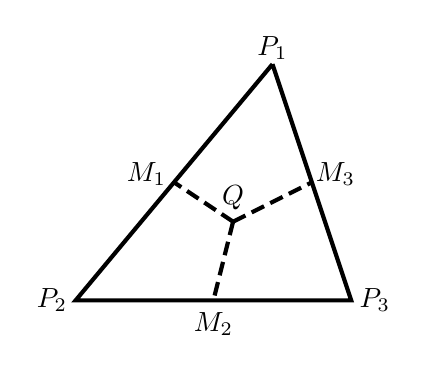
\begin{tikzpicture}[>=stealth]
		 \draw[dash pattern = on 5pt off 2.5pt, line width = 1.5pt] (0,0) --  (-0.75,0.5);
		 \draw[dash pattern = on 5pt off 2.5pt, line width = 1.5pt] (0,0) -- (-0.25,-1);
		 \draw[dash pattern = on 5pt off 2.5pt, line width = 1.5pt] (0,0) -- (1,0.5);
         %%%%%%%%%%%%%%%%%%%%%%%%%%%%%%%%%%%%%%%%%%%%%%%%%%%
        \draw[line width = 1.5pt] (0.5,2) to (-2,-1) to (1.5,-1) to (0.5,2);
         %%%%%%%%%%%%%%%%%%%%%%%%%%%%%%
         %\node at (0,0) {\TeX};
         %\node [<options>] (<name>) at(<coordinate>){<node contents>};
         \node at (0,0.3){$Q$};
         \node at (0.5,2.2){$P_1$};
         \node at (-2.3,-1){$P_2$};
         \node at (1.8,-1){$P_3$};
         \node at (-1.1,0.6){$M_1$};
         \node at (-0.25,-1.3){$M_2$};
         \node at (1.3,0.6){$M_3$};
        \end{tikzpicture}
		\caption{Triangle element $K_Q$ ($\triangle P_{1}P_{2}P_{3}$).}
  \label{Fig2}
\end{figure}	

For each triangular element $K_Q$ (\Cref{Fig2}) in the triangulation $T_h$,
the following equality holds \cite{lironghua}
\begin{equation}
\begin{aligned}
    \frac{\partial \tilde{\bmf{m}}_h}{\partial x}
    & =  \frac{1}{2S_{K_Q}}
    \sum_{i=1}^3 \tilde{\bmf{m}}_h(P_i)(y_{M_{i}}-y_{M_{i+2}}),\\
    \frac{\partial \tilde{\bmf{m}}_h}{\partial y}
    & =   \frac{1}{2S_{K_Q}}
    \sum_{i=1}^3 \tilde{\bmf{m}}_h(P_i)(x_{M_{i+2}}-x_{M_i}),
    \label{triangle_area}
\end{aligned}
\end{equation}
where $S_{K_Q}$ is the area of triangle element $K_Q$, $ \ M_4 = M_1$ and $\ M_5 = M_2$.
Since $ \frac{\partial \tilde{\bmf{m}}_h}{\partial x} $ and $ \frac{\partial\tilde{\bmf{m}}_h}{\partial y}$ are constants in the triangular element $K_Q$,
we have
\begin{equation*}
\begin{aligned}
& I_{K_Q} (\bmf{\Phi};\tilde{\bmf{m}}_h,I_h^*\tilde{\bmf{m}}_h)\\ \nn
 =
 & \sum_{i=1}^3 \tilde{\bmf{m}}_h(P_i) \cdot \int_{\overline{M_iQM_{i+2}}} \bmf{\Phi} \times \frac{\partial \tilde{\bmf{m}}_h(Q)}{\partial \bmf{\nu}} \,\mr{d}S \\
=
& \sum_{i=1}^3 \tilde{\bmf{m}}_h(P_i) \cdot \left[ \int_{\overline{M_iQM_{i+2}}} \bmf{\Phi} \times \frac{\partial \tilde{\bmf{m}}_h(Q)}{\partial x} \,\mr{d}y
- \int_{\overline{M_iQM_{i+2}}} \bmf{\Phi} \times \frac{\partial \tilde{\bmf{m}}_h(Q)}{\partial y} \, \mr{d}x \right] \\
=
& \sum_{i=1}^3 \tilde{\bmf{m}}_h(P_i) \cdot \left[ \left(\bmf{\Phi} \times \frac{\partial \tilde{\bmf{m}}_h(Q)}{\partial x}\right) (y_{M_{i+2}}-y_{M_i})
- \left(\bmf{\Phi} \times \frac{\partial \tilde{\bmf{m}}_h(Q)}{\partial y}\right) (x_{M_{i+2}}-x_{M_i})\right]\\ \nn
=
& - 2 S_{K_Q} \left[\left(\bmf{\Phi} \times \frac{\partial \tilde{\bmf{m}}_h(Q)}{\partial x}\right) \cdot \frac{\partial \tilde{\bmf{m}}_h(Q)}{\partial x} + \left(\bmf{\Phi} \times \frac{\partial \tilde{\bmf{m}}_h(Q)}{\partial y}\right) \cdot \frac{\partial \tilde{\bmf{m}}_h(Q)}{\partial y}\right]\\ \nn
=
& 0.
\end{aligned}
\end{equation*}
It therefore holds $b_h(\bmf{\Phi};\tilde{\bmf{m}}_h,I_h^*\tilde{\bmf{m}}_h) =  0$.
% \begin{equation*}
% b_h(\bmf{\Phi};\tilde{\bmf{m}}_h,I_h^*\tilde{\bmf{m}}_h) =  0.
% \end{equation*}

Next, we estimate the bound of $b_h(\bmf{\Phi};\cdot,I_h^{*}\cdot)$.
\begin{equation*}
\begin{aligned}
&  I_{K_Q} (\bmf{\Phi};\tilde{\bmf{m}}_h,I_h^*\bmf{v}_h)\\ \nn
=
& - \sum_{i=1}^3 \bmf{v}_h(P_1)\cdot\int_{\overline{M_iQM_{i+2}}} \bmf{\Phi}\times \frac{\partial \tilde{\bmf{m}}_h}{\partial \bmf{\nu}} \, \mr{d}S
\\
=
& \sum_{i=1}^3  (\bmf{v}_h(P_{i+1})-\bmf{v}_h(P_i))\cdot\int_{\overline{M_iQ}}\bmf{\Phi}\times \frac{\partial \tilde{\bmf{m}}_h}{\partial \bmf{\nu}} \, \mr{d}S,
\end{aligned}
\end{equation*}
where $ P_4 = P_1 $. Denote $l_i=|\overline{P_{i}P_{i+1}}|$,
$\tau_i=\frac{\overrightarrow{P_{i}P_{i+1}}}{l_i}$, ($ i = 1,2,3 $), and
% Combining with the linearity of $ \bmf{v}_h $ over the triangular element $ K_Q $,
we have
\begin{equation*}
\frac{\bmf{v}_h(P_{i+1})-\bmf{v}_h(P_{i})}{l_i}
=
\frac{\partial \bmf{v}_h}{\partial \tau_i}.
\end{equation*}
% Therefore,
% \begin{equation*}
% \begin{aligned}
% I_{K_Q}(\bmf{\Phi};\tilde{\bmf{m}}_h,I_h^*\bmf{v}_h)
% =
% \sum_{i=1}^{3} l_i \int_{\overline{M_i Q}}\bmf{\Phi}\times \frac{\partial \tilde{\bmf{m}}_h}{\partial \bmf{\nu}} \frac{\partial \bmf{v}_h}{\partial \tau_i} \,\mr{d}S.
% \end{aligned}
% \end{equation*}
We then arrive at
\begin{equation*}
\begin{aligned}
& b_h(\bmf{\Phi};\tilde{\bmf{m}}_h,I_h^*\bmf{v}_h)\\
 = &
 \sum_{{K_Q}\in T_h} \sum_{i=1}^{3} l_i \int_{\overline{M_i Q}}\left(\bmf{\Phi}\times \frac{\partial \tilde{\bmf{m}}_h}{\partial \bmf{\nu}}\right)\cdot \frac{\partial \bmf{v}_h}{\partial \tau_i} \,\mr{d}S\\
 \leq &
\sum_{{K_Q}\in T_h} \sum_{i=1}^{3} l_i |\bmf{\Phi}(Q)| \left|\frac{\partial \tilde{\bmf{m}}_h(Q)}{\partial \bmf{\nu}}\right| \left|\frac{\partial \bmf{v}_h(Q)}{\partial \tau_i}\right| |\overline{M_i Q}|\\
 \leq & \
C \sum_{{K_Q}\in T_h} h^2
\left(\left|\frac{\partial \tilde{\bmf{m}}_h(Q)}{\partial x}\right| + \left|\frac{\partial \tilde{\bmf{m}}_h(Q)}{\partial y}\right|\right)
\left(\left|\frac{\partial \bmf{v}_h(Q)}{\partial x}\right| + \left|\frac{\partial \bmf{v}_h(Q)}{\partial y} \right|\right) \\
 \leq & \
C \,\| \tilde{\bmf{m}}_h \|_{\bmf{H}^1}  \| \bmf{v}_h \|_{\bmf{H}^1}.
\end{aligned}
\end{equation*}
\end{proof}
By Lemma \ref{lem-ah} and Lemma \ref{lem-bh},
we get
\begin{equation*}
\begin{aligned}
&\mathcal{A}_h(\bmf{\Phi};\tilde{\bmf{m}}_h,I_h^*\tilde{\bmf{m}}_h)
=
a_h(\tilde{\bmf{m}}_h,I_h^*\tilde{\bmf{m}}_h)
+
b_h(\bmf{\Phi};\tilde{\bmf{m}}_h,I_h^*\tilde{\bmf{m}}_h)
\geq
C \|\tilde{\bmf{m}}_h\|_{\bmf{H}^1}^2,\\
&|\mathcal{A}_h(\bmf{\Phi};\tilde{\bmf{m}}_h,I_h^*\bmf{v}_h)|
\leq
|a_h(\tilde{\bmf{m}}_h,I_h^*\bmf{v}_h)|+|b_h(\bmf{\Phi};\tilde{\bmf{m}}_h,I_h^*\bmf{v}_h)|
\leq
C \| \tilde{\bmf{m}}_h \|_{\bmf{H}^1}  \| \bmf{v}_h \|_{\bmf{H}^1}.
\end{aligned}
\end{equation*}
These complete the proof.


\section{The proof of Lemma \ref{lem-Ah1}}\label{app:lem-Ah1}
Repeat the proof of Lemma 2.4 in \cite{chou},
we obtain
\begin{equation}
|a_h(\tilde{\bmf{m}}_h,I_h^*\bmf{v}_h)-a_h(\bmf{v}_h,I_h^*\tilde{\bmf{m}}_h)|
\leq
C h\|\tilde{\bmf{m}}_h\|_{\bmf{H}^1}\|\bmf{v}_h\|_{\bmf{H}^1}, \quad \forall \tilde{\bmf{m}}_h,\bmf{v}_h\in \bmf{S}_h.
\label{ah-relation}
\end{equation}
Hence,
we focus solely on estimating the bound of $|b_h(\bmf{\Phi};\tilde{\bmf{m}}_h,I_h^*\bmf{v}_h) - b_h(\bmf{\Phi};\bmf{v}_h,I_h^*\tilde{\bmf{m}}_h)|$.

For $\tilde{\bmf{m}}\in \bmf{H}^2$, $\tilde{\bmf{m}}_h,\bmf{v}_h \in \bmf{S}_h$,
applying Green formula yields
\begin{equation}
\begin{aligned}
 b(\bmf{\Phi};\tilde{\bmf{m}}-\tilde{\bmf{m}}_h,\bmf{v}_h)
    = &
   -\sum_{K_Q\in T_h} \int_{K_Q} \left(\bmf{\Phi}\times\nabla(\tilde{\bmf{m}}-\tilde{\bmf{m}}_h)\right) \cdot \nabla\bmf{v}_h \, \mr{d}x\mr{d}y \\
    = &
    -\sum_{K_Q\in T_h} \int_{K_Q} \left((\bmf{\Phi}\!-\!\bmf{\Phi}(Q))\times\nabla(\tilde{\bmf{m}}-\tilde{\bmf{m}}_h)\right) \cdot \nabla\bmf{v}_h \mr{d}x\mr{d}y \\
   & +
   \sum_{K_Q\in T_h} \int_{K_Q} \left(\bmf{\Phi}(Q)\times\Delta \tilde{\bmf{m}}\right) \cdot \bmf{v}_h \, \mr{d}x\mr{d}y\\
   & -
   \sum_{K_Q\in T_h} \int_{K_Q} \left(\nabla\bmf{\Phi}(Q)\times\nabla \tilde{\bmf{m}}\right) \cdot \bmf{v}_h \, \mr{d}x\mr{d}y\\
   & +
   \int_{\partial{K_Q}} \left(\bmf{\Phi}(Q)\times \frac{\partial(\tilde{\bmf{m}}-\tilde{\bmf{m}}_h)}{\partial\bmf{\nu}}\right) \cdot\bmf{v}_h \, \mr{d}S.
\end{aligned}
\label{b-1}
\end{equation}
Meanwhile, for $\tilde{\bmf{m}}\in \bmf{H}^2$, $\bmf{v}_h \in \bmf{S}_h$, we have
\begin{equation*}
\begin{aligned}
   & \sum_{K_Q \in T_h} \int_{K_Q} \left(\bmf{\Phi}(Q)\times\Delta \tilde{\bmf{m}}\right) \cdot \bmf{v}_h \, \mr{d}x\mr{d}y \\
   = &
   \sum_{K_Q \in T_h} \sum_{P\in \dot{K}_Q} \int_{{K_Q} \bigcap V_i} \left(\bmf{\Phi}(Q)\times\Delta \tilde{\bmf{m}}\right) \cdot \bmf{v}_h \, \mr{d}x\mr{d}y\\
   = &
   \sum_{K_Q \in T_h} \sum_{P\in \dot{K}_Q} \left[\int_{\partial({K_Q} \bigcap V_i)} \left(\bmf{\Phi}(Q)\times \frac{\partial\tilde{\bmf{m}}}{\partial\bmf{\nu}}\right) \cdot\bmf{v}_h \, \mr{d}S
   -
   \int_{{K_Q} \bigcap V_i} \left(\nabla\bmf{\Phi}(Q)\times\nabla \tilde{\bmf{m}}\right) \cdot\bmf{v}_h \, \mr{d}x\mr{d}y \right]\\
   % =  &
   % \sum_{K_Q \in T_h} \sum_{P\in \dot{K}_Q} (\int_{\partial V_i \bigcap {K_Q}} \bmf{\Phi}(Q)\times(\frac{\partial\tilde{\bmf{m}}}{\partial\bmf{\nu}}) \bmf{v}_h \, \mr{d}S
   % -
   % \int_{{K_Q} \bigcap V_i} (\nabla\bmf{\Phi}(Q)\times\nabla \tilde{\bmf{m}}) \bmf{v}_h \, \mr{d}x\mr{d}y)\\
   % & +
   % \sum_{K_Q \in T_h} \int_{\partial{K_Q}} (\bmf{\Phi}(Q)\times(\frac{\partial\tilde{\bmf{m}}}{\partial\bmf{\nu}}) \bmf{v}_h \, \mr{d}S\\
   =  &
   \sum_{K_Q \in T_h} \sum_{P\in \dot{K}_Q} \int_{\partial V_i \bigcap {K_Q}} \left(\bmf{\Phi}(Q)\times \frac{\partial\tilde{\bmf{m}}}{\partial\bmf{\nu}}\right) \cdot\bmf{v}_h \, \mr{d}S
   -
    \sum_{K_Q \in T_h}\int_{{K_Q}} \left(\nabla\bmf{\Phi}(Q)\times\nabla \tilde{\bmf{m}}\right) \cdot \bmf{v}_h \, \mr{d}x\mr{d}y\\
   & +
   \sum_{K_Q \in T_h} \int_{\partial{K_Q}} \left(\bmf{\Phi}(Q)\times \frac{\partial\tilde{\bmf{m}}}{\partial\bmf{\nu}}\right)  \cdot \bmf{v}_h \, \mr{d}S.
\end{aligned}
% \label{bh-la}
\end{equation*}
Let $\bmf{v}_h = I_h^*\bmf{v}_h$ in \eqref{b-1} and we obtain
\begin{equation*}
\begin{aligned}
 b_h(\bmf{\Phi};\tilde{\bmf{m}}-\tilde{\bmf{m}}_h,I_h^*\bmf{v}_h)
    = &
   \sum_{K_Q \in T_h} \sum_{P\in \dot{K}_Q}  \int_{\partial V_i \bigcap K_Q} \left(\bmf{\Phi}\times \frac{\partial(\tilde{\bmf{m}}-\tilde{\bmf{m}}_h)}{\partial\bmf{\nu}}\right) \cdot I_h^*\bmf{v}_h \, \mr{d}S \\
    = &
   \sum_{K_Q \in T_h} \sum_{P\in \dot{K}_Q}  \int_{\partial V_i \bigcap K_Q} \left(\left(\bmf{\Phi}-\bmf{\Phi}(Q)\right)\times \frac{\partial(\tilde{\bmf{m}}-\tilde{\bmf{m}}_h)}{\partial\bmf{\nu}}\right) \cdot I_h^*\bmf{v}_h \, \mr{d}S   \\
   & +
   \sum_{K_Q\in T_h}\int_{K_Q} \left(\bmf{\Phi}(Q)\times\Delta \tilde{\bmf{m}}\right) \cdot I_h^*\bmf{v}_h \, \mr{d}x\mr{d}y\\
   &
   -
   \sum_{K_Q\in T_h}\int_{K_Q} \left(\nabla\bmf{\Phi}(Q)\times\nabla \tilde{\bmf{m}}\right) \cdot I_h^*\bmf{v}_h \, \mr{d}x\mr{d}y\\
  & +
   \sum_{K_Q\in T_h}\int_{\partial{K_Q}} \left(\bmf{\Phi}(Q)\times \frac{\partial(\tilde{\bmf{m}}-\tilde{\bmf{m}}_h)}{\partial\bmf{\nu}}\right) \cdot I_h^*\bmf{v}_h \, \mr{d}S.
\end{aligned}
\end{equation*}
Hence, we have
\begin{equation*}
     b(\bmf{\Phi};\tilde{\bmf{m}}-\tilde{\bmf{m}}_h,\bmf{v}_h) - b_h(\bmf{\Phi};\tilde{\bmf{m}}-\tilde{\bmf{m}}_h,I_h^*\bmf{v}_h)
     =
     \sum_{i=1}^5 E_i(\bmf{\Phi};\tilde{\bmf{m}}-\tilde{\bmf{m}}_h,\bmf{v}_h),
\end{equation*}
where
\begin{equation*}
     E_1(\bmf{\Phi};\tilde{\bmf{m}}-\tilde{\bmf{m}}_h,\bmf{v}_h)
     =
     -\sum_{K_Q\in T_h} \int_{K_Q} \left((\bmf{\Phi}\!-\!\bmf{\Phi}(Q))\times\nabla(\tilde{\bmf{m}}-\tilde{\bmf{m}}_h)\right) \cdot \nabla\bmf{v}_h \mr{d}x\mr{d}y,
\end{equation*}
\begin{equation*}
    E_2(\bmf{\Phi};\tilde{\bmf{m}}-\tilde{\bmf{m}}_h,\bmf{v}_h)
    =
    \sum_{K_Q \in T_h} \sum_{P\in \dot{K}_Q}  \int_{\partial V_i \bigcap K_Q} \left(\bmf{\Phi}\times \frac{\partial(\tilde{\bmf{m}}-\tilde{\bmf{m}}_h)}{\partial\bmf{\nu}} \right) \cdot I_h^*\bmf{v}_h \, \mr{d}S,
\end{equation*}
\begin{equation*}
    E_3(\bmf{\Phi};\tilde{\bmf{m}}-\tilde{\bmf{m}}_h,\bmf{v}_h)
    =
     \sum_{K_Q\in T_h} \int_{K_Q} (\bmf{\Phi}(Q)\times\Delta \tilde{\bmf{m}}) \cdot (\bmf{v}_h-I_h^*\bmf{v}_h) \, \mr{d}x\mr{d}y,
\end{equation*}
\begin{equation*}
    E_4(\nabla\bmf{\Phi};\tilde{\bmf{m}}-\tilde{\bmf{m}}_h,\bmf{v}_h)
    =
    -\sum_{K_Q\in T_h} \int_{K_Q} (\nabla\bmf{\Phi}(Q)\times\nabla \tilde{\bmf{m}}) \cdot
    (\bmf{v}_h-I_h^*\bmf{v}_h) \, \mr{d}x\mr{d}y,
\end{equation*}
\begin{equation*}
    E_5(\bmf{\Phi};\tilde{\bmf{m}}-\tilde{\bmf{m}}_h,\bmf{v}_h)
    =
    \int_{\partial{K_Q}} \left(\bmf{\Phi}(Q)\times \frac{\partial(\tilde{\bmf{m}}-\tilde{\bmf{m}}_h)}{\partial\bmf{\nu}}\right) \cdot (\bmf{v}_h-I_h^*\bmf{v}_h) \, \mr{d}S.
\end{equation*}
We next derive the bounds of $E_i$.
For $E_1$, since $\bmf{\Phi} \in \bmf{X}$, it holds
\begin{equation*}
    |E_1(\bmf{\Phi};\tilde{\bmf{m}}-\tilde{\bmf{m}}_h,\bmf{v}_h)| \leq C h \|\tilde{\bmf{m}}-\tilde{\bmf{m}}_h\|_{\bmf{H}^1}\|\bmf{v}_h\|_{\bmf{H}^1}.
\end{equation*}
$E_2(\bmf{\Phi};\tilde{\bmf{m}}-\tilde{\bmf{m}}_h,\bmf{v}_h)$ can be rewritten into
\begin{equation*}
\left|E_2(\bmf{\Phi};\tilde{\bmf{m}}-\tilde{\bmf{m}}_h,\bmf{v}_h) \right|
=
 \left|\sum_{K_Q \in T_h} \sum_{i=1}^3  (\bmf{v}_h(P_{i+1})-\bmf{v}_h(P_i))\cdot\int_{\overline{M_iQ}}(\bmf{\Phi}-\bmf{\Phi}(Q))\times \frac{\partial(\tilde{\bmf{m}}- \tilde{\bmf{m}}_h)}{\partial \bmf{\nu}} \, \mr{d}S\right|,
\end{equation*}
where $P_i$ denotes the vertex of triangle element $K_Q$, and $P_4=P_1$. Since $\bmf{v}_h$ is linear in $K_Q$, and using the Taylor's expansion, we get
\begin{equation*}
    |\bmf{v}_h(P_{i+1})-\bmf{v}_h(P_i)|
    =
    \left|\frac{\partial\bmf{v}_h}{\partial x} (x_{P_i}-x_{P_{i+1}})+ \frac{\partial\bmf{v}_h}{\partial y} (y_{P_i}-y_{P_{i+1}}) \right|
    \leq
    h \left(\left|\frac{\partial\bmf{v}_h}{\partial x}\right| + \left| \frac{\partial\bmf{v}_h}{\partial y} \right|\right).
\end{equation*}
Combined with the inequality \cite{chou}
\begin{equation*}
    \int_{\overline{M_iQ}} \left( \frac{\partial(\tilde{\bmf{m}}- \tilde{\bmf{m}}_h)}{\partial \bmf{\nu}}\right)^2 \, \mr{d}S
    \leq
    C(h^{-1} |\tilde{\bmf{m}} - \tilde{\bmf{m}}_h|_{\bmf{H}^1(K_Q)}^2 + |\tilde{\bmf{m}}|_{\bmf{H}^2(K_Q)}|\tilde{\bmf{m}} - \tilde{\bmf{m}}_h|_{\bmf{H}^1(K_Q)}),
\end{equation*}
it leads to an estimate
\begin{equation*}
    \begin{aligned}
& |E_2(\bmf{\Phi};\tilde{\bmf{m}}-\tilde{\bmf{m}}_h,\bmf{v}_h)|\\
\leq &
 \sum_{K_Q \in T_h} \sum_{i=1}^3  |\bmf{v}_h(P_{i+1})-\bmf{v}_h(P_i)|\int_{\overline{M_iQ}}|\bmf{\Phi}-\bmf{\Phi}(Q)| \left|\frac{\partial(\tilde{\bmf{m}}- \tilde{\bmf{m}}_h)}{\partial \bmf{\nu}}\right| \, \mr{d}S\\
  \leq &
 C h (\|\tilde{\bmf{m}}-\tilde{\bmf{m}}_h\|_{\bmf{H}^1}+h^{1/2}\|\tilde{\bmf{m}}-\tilde{\bmf{m}}_h\|_{\bmf{H}^1}^{1/2}\|\tilde{\bmf{m}}\|_{\bmf{H}^2}^{1/2})\|\bmf{v}_h\|_{\bmf{H}^1}.
\end{aligned}
\end{equation*}
Owing to
\begin{equation*}
    \|\bmf{v}_h-I_h^*\bmf{v}_h\|_{\bmf{L}^2} \leq h \|\bmf{v}_h\|_{\bmf{H}^1},
    \, \forall \, \bmf{v}_h \in \bmf{S}_h,
\end{equation*}
we obtain
\begin{equation*}
    |E_3(\bmf{\Phi};\tilde{\bmf{m}}-\tilde{\bmf{m}}_h,\bmf{v}_h)| \leq C h \|\tilde{\bmf{m}}\|_{\bmf{H}^2}\|\bmf{v}_h\|_{\bmf{H}^{1}},
\end{equation*}
and
\begin{equation*}
    |E_4(\nabla\bmf{\Phi};\tilde{\bmf{m}}-\tilde{\bmf{m}}_h,\bmf{v}_h)|
    \leq C h \|\tilde{\bmf{m}}\|_{\bmf{H}^1}\|\bmf{v}_h\|_{\bmf{H}^{1}}.
\end{equation*}
Since $ \frac{\partial\bmf{v}_h}{\partial\bmf{\nu}} $ is a constant along with edges of the element $K_Q$, i.e.,
\begin{equation}
    \int_{\partial K_Q}(\bmf{v}_h-I_h^*\bmf{v}_h)\,\mr{d}S = 0,
    \label{pk}
\end{equation}
for $E_5$, we have
\begin{equation*}
\begin{aligned}
    E_5(\bmf{\Phi};\tilde{\bmf{m}}-\tilde{\bmf{m}}_h,\bmf{v}_h)
    =&
    \int_{\partial{K_Q}} \left(\bmf{\Phi}(Q)\times \frac{\partial(\tilde{\bmf{m}}-\tilde{\bmf{m}}_h)}{\partial\bmf{\nu}}\right) \cdot (\bmf{v}_h-I_h^*\bmf{v}_h) \, \mr{d}S\\
    =&
    \int_{\partial{K_Q}} \left(\bmf{\Phi}(Q)\times \frac{\partial\tilde{\bmf{m}}}{\partial\bmf{\nu}}\right) \cdot (\bmf{v}_h-I_h^*\bmf{v}_h) \, \mr{d}S.
\end{aligned}
\end{equation*}
Let $N_e$ denote the number of all triangle elements $K_Q$, and let $L$ denote the common edge shared by $K_{Q_i}$ and $K_{Q_{i+1}}$.
Then, we have
\begin{equation*}
\begin{aligned}
    E_5(\bmf{\Phi};\tilde{\bmf{m}}-\tilde{\bmf{m}}_h,\bmf{v}_h)
    = &
    \sum_{i=1}^{N_e}\int_{L}
    \left(\left(\bmf{\Phi}(Q_{i+1})-\bmf{\Phi}(Q_i)\right)\times \frac{\partial\tilde{\bmf{m}}}{\partial\bmf{\nu}}\right) \cdot \left(\bmf{v}_h-I_h^*\bmf{v}_h\right) \, \mr{d}S\\
    = &
    \sum_{i=1}^{N_e}\int_{L}
    \left(\left(\bmf{\Phi}(Q_{i+1})-\bmf{\Phi}(Q_i)\right)\times \left( \frac{\partial\tilde{\bmf{m}}}{\partial\bmf{\nu}}-C_m\right)\right) \cdot\left(\bmf{v}_h-I_h^*\bmf{v}_h\right) \, \mr{d}S,
\end{aligned}
\end{equation*}
where $C_m$ is a constant defined as
\begin{equation*}
    C_m := \frac{1}{2} \left( \frac{\partial\tilde{\bmf{m}}_h^{i}}{\partial \bmf{\nu}}+\frac{\partial\tilde{\bmf{m}}_h^{i+1}}{\partial \bmf{\nu}} \right)
\end{equation*}
with $\tilde{\bmf{m}}_h^{i}$ and $\tilde{\bmf{m}}_h^{i+1}$ being the bounds of $\tilde{\bmf{m}}_h$ in the triangular element $K_{Q_i}$ and $K_{Q_{i+1}}$, respectively.
Consequently, we obtain
\begin{equation*}
\begin{aligned}
    E_5(\bmf{\Phi};\tilde{\bmf{m}}-\tilde{\bmf{m}}_h,\bmf{v}_h)
    = &
    \sum_{i=1}^{N_e}\int_{L}
    \left(\left(\bmf{\Phi}(Q_{i+1})-\bmf{\Phi}(Q_i)\right)\times \left( \frac{\partial\tilde{\bmf{m}}}{\partial \bmf{\nu}}-\frac{\partial\tilde{\bmf{m}}_h^k}{\partial \bmf{\nu}}\right)\right)\cdot (\bmf{v}_h-I_h^*\bmf{v}_h) \, \mr{d}S,
\end{aligned}
\end{equation*}
where $k = i \,\mr{or}\, i+1$.

Owing to the inequality \cite{chou}
\begin{equation*}
    \left( \int_{\partial K_Q}(\bmf{v}_h-I_h^*\bmf{v}_h)^2\,\mr{d}S \right)^{\frac{1}{2}} \leq C h^{\frac{1}{2}}\|\bmf{v}_h\|_{\bmf{H}^1},
\end{equation*}
we obtain
\begin{equation*}
 |E_5(\bmf{\Phi};\tilde{\bmf{m}}-\tilde{\bmf{m}}_h,\bmf{v}_h)|
 \leq
 C h (\|\tilde{\bmf{m}}-\tilde{\bmf{m}}_h\|_{\bmf{H}^1}+h^{1/2}\|\tilde{\bmf{m}}-\tilde{\bmf{m}}_h\|_{\bmf{H}^1}^{1/2}\|\tilde{\bmf{m}}\|_{\bmf{H}^2}^{1/2})\|\bmf{v}_h\|_{\bmf{H}^1}.
\end{equation*}
Together with triangle inequality, it yields
\begin{equation}
|b_h(\bmf{\Phi};\tilde{\bmf{m}}_h,I_h^*\bmf{v}_h) - b_h(\bmf{\Phi};\bmf{v}_h,I_h^*\tilde{\bmf{m}}_h)|
\leq
C h \|\tilde{\bmf{m}}_h\|_{\bmf{H}^1}\|\bmf{v}_h\|_{\bmf{H}^1}, \quad \forall \tilde{\bmf{m}}_h,\bmf{v}_h\in \bmf{S}_h.
\label{bh-relation}
\end{equation}
These complete the proof.


\section{The proof of Lemma \ref{erfunction}}\label{app:lem-erfun}
To prove Lemma \ref{erfunction}, we denote
$\mathcal{A}_h(\bmf{\Phi};R_h\tilde{\bmf{m}}_h,\bmf{v}_h) = \varepsilon_a (R_h\tilde{\bmf{m}},\bmf{v}_h) - \varepsilon_b(\bmf{\Phi};R_h\tilde{\bmf{m}}_h,\bmf{v}_h)$ with
\begin{equation*}
   \varepsilon_a (R_h\tilde{\bmf{m}},\bmf{v}_h)= a(R_h\tilde{\bmf{m}},\bmf{v}_h)-a_h(R_h\tilde{\bmf{m}}_h,I_h^*\bmf{v}_h), \,\forall \bmf{m}_h,\bmf{v}_h\in \bmf{S}_h,
\end{equation*}
and
\begin{equation*}
\varepsilon_b(\bmf{\Phi};R_h\tilde{\bmf{m}}_h,\bmf{v}_h)
=
b(\bmf{\Phi};R_h\tilde{\bmf{m}}_h,\bmf{v}_h)
-
b_h(\bmf{\Phi};R_h\tilde{\bmf{m}}_h,I_h^*\bmf{v}_h),\,\forall \bmf{m}_h,\bmf{v}_h\in \bmf{S}_h.
\end{equation*}

Repeat the proof as in \cite{chat1,chat2}, we get
\begin{equation*}
|\varepsilon_h(\bmf{f},\bmf{v}_h)|
\leq
Ch^{i+j}\|\bmf{f}\|_{\bmf{H}^i}\|\bmf{v}_h\|_{\bmf{H}^j},
\quad
\bmf{f}\in \bmf{H}^i, i,j=0,1, \, \bmf{v}_h\in \bmf{S}_h,
\end{equation*}
and
\begin{equation}
|\varepsilon_a(R_h \tilde{\bmf{m}},\bmf{v}_h)|
\leq Ch^{i+j}\|\tilde{\bmf{m}}\|_{\bmf{H}^{1+i}}\|\bmf{v}_h\|_{\bmf{H}^j},
\quad
\tilde{\bmf{m}}\in \bmf{H}^{1+i}\cap \bmf{H}^1_0,i,j=0,1,\,\bmf{v}_h\in \bmf{S}_h.
\label{erfun-a1}
\end{equation}
For the bound of $|\varepsilon_b(\bmf{\Phi};R_h \tilde{\bmf{m}},\bmf{v}_h)|$,
we consider the linear operator
$$L_1|_{K_Q} : \bmf{P}_1(K_Q) \rightarrow \bmf{L}^2(K_Q), \quad K_Q \in T_h, $$
that satisfies $\int_{K_Q} L_1 C \mr{d} x \mr{d} y= \int_{K_Q} C \mr{d} x\mr{d}y$.
Then for all constants $C$ and $K_Q \in T_h$,
\begin{equation}
    \|\bmf{v}_h-L_1\bmf{v}_h\|_{\bmf{L}^q(K_Q)} \leq h_{K_Q} |\bmf{v}_h|_{\bmf{W}^{1,q}(K_Q)},
    \, \forall \, \bmf{v}_h \in \bmf{S}_h, \, 1 \leq q < \infty.
    \label{L1}
\end{equation}
Meanwhile, consider the linear operator
$$L_2|_{\partial K_Q} : \bmf{P}_1(K_Q) \rightarrow \bmf{L}^2(\partial K_Q),$$
which has the properties
\begin{equation*}
    L_2 C |_{\partial K_Q} = C, \quad \mr{for \, all \, constants} \, C,
    \label{L21}
\end{equation*}
\begin{equation*}
    \int_{\partial K_Q} \bmf{v}_h \, \mr{d} S = \int_{\partial K_Q} L_2 \bmf{v}_h \, \mr{d}S,
    \quad   \forall \, \bmf{v}_h \,\in \bmf{P}_1(K_Q),
\label{L22}
\end{equation*}
\begin{equation*}
    \|L_2 \bmf{v}_h\|_{\bmf{L}^{\infty}(\partial K_Q)} \leq \|\bmf{v}_h\|_{\bmf{L}^{\infty}(\partial K_Q)},
    \, \forall \bmf{v}_h \, \in \, \bmf{S}_h.
    \label{L23}
\end{equation*}
Repeat the proof of Lemma 6.1 in \cite{chat2}, we can obtain:
Given $ \bmf{\Phi} \in \bmf{X}$,
for arbitrary triangle element $K_Q$,
there exists a constant $C$ independent of $K_Q$ such that
\begin{equation*}
    \left|\int_{\partial K_Q} (\bmf{\Phi} \times \nabla R_h\tilde{\bmf{m}})\cdot(\bmf{v}_h-L_2\bmf{v}_h) \,\mr{d}S \right|
    \leq C h_{K_Q} |\tilde{\bmf{m}}|_{\bmf{H}^1(K_Q)}|\bmf{v}_h|_{\bmf{H}^1(K_Q)},
    \quad \forall\,\bmf{m} \in \bmf{H}^1(K_Q), \, \bmf{v}_h \in \bmf{S}_h.
    \label{L11}
\end{equation*}
Applying Green's formula, we obtain
\begin{equation}
\begin{aligned}
    \varepsilon_b(\bmf{\Phi};R_h\tilde{\bmf{m}},\bmf{v}_h)
    =&
    \sum_{K_Q} (\mr{div}(\bmf{\Phi} \times \nabla R_h\tilde{\bmf{m}}), \bmf{v}_h - L_1 \bmf{v}_h)_{K_Q}\\
    & +
    \sum_{K_Q} (\bmf{\Phi} \times (\nabla R_h \tilde{\bmf{m}} \cdot \bmf{n}), \bmf{v}_h - L_2 \bmf{v}_h)_{\partial K_Q}\\
    :=&
    J_1 + J_2.
\end{aligned}
\label{erfun-b1}
\end{equation}
For each triangular element $K_Q$, applying Green's formula yields
\begin{equation*}
\begin{aligned}
     &\int_{K_Q}\mr{div}(\bmf{\Phi} \times \nabla R_h\tilde{\bmf{m}})\, \mr{d}x\mr{d}y\\
    =&
    \sum_{V_i}\int_{V_i \bigcap K_Q} \mr{div}(\bmf{\Phi} \times \nabla R_h\tilde{\bmf{m}}) \, \mr{d}x\mr{d}y\\
    =&
    -\sum_{V_i}\int_{\partial V_i \bigcap K_Q}(\bmf{\Phi} \times \nabla R_h\tilde{\bmf{m}})\cdot \bmf{n} \, \mr{d}S
    -\sum_{V_i}\int_{V_i \bigcap \partial K_Q}(\bmf{\Phi} \times \nabla R_h\tilde{\bmf{m}})\cdot \bmf{n} \, \mr{d}S.
\end{aligned}
\end{equation*}
Combined with \eqref{L1} and H\"{o}lder inequality, we obtain
\begin{equation}
    |J_1|
    \leq C \sum_{K_Q} \|\mr{div}(\bmf{\Phi} \times \nabla\tilde{\bmf{m}})\|_{\bmf{L}^2(K_Q)}\| \bmf{v}_h - L_1 \bmf{v}_h\|_{\bmf{L}^2(K_Q)}
    \leq C \sum_{K_Q} h_{K_Q} |\tilde{\bmf{m}}|_{\bmf{H}^1(K_Q)}|\bmf{v}_h|_{\bmf{H}^1(K_Q)}.
    \label{J1}
\end{equation}
Meanwhile, since $|\bmf{\Phi} \times (\nabla R_h \tilde{\bmf{m}} \cdot \bmf{n})|_{\bmf{H}^1(K_Q)} \leq C |\tilde{\bmf{m}}|_{\bmf{H}^1(K_Q)}$, it holds
\begin{equation}
    |J_2| \leq C \sum_{K_Q} h_{K_Q} |\tilde{\bmf{m}}|_{\bmf{H}^1(K_Q)}|\bmf{v}_h|_{\bmf{H}^1(K_Q)}.
    \label{J2}
\end{equation}
Summing the inequalities \eqref{erfun-b1}-\eqref{J2} yields
\begin{equation}
|\varepsilon_b(\bmf{\Phi};R_h\tilde{\bmf{m}},\bmf{v}_h)|
\leq Ch^{i+j}\|\tilde{\bmf{m}}\|_{\bmf{H}^{1+i}}\|\bmf{v}_h\|_{\bmf{H}^j},
\quad
\bmf{v}\in \bmf{H}^{1+i}\cap \bmf{H}^1_0,i,j=0,1.
\label{erfun-b}
\end{equation}
Together with \eqref{erfun-b} and \eqref{erfun-a1}, it yields \eqref{erfun-A1}.

\section{The proof of Proposition \ref{lem-t}}\label{app:lem-ah-t}
We rewrite $a_h(\bmf{m}_h,I_h^*\partial_t\bmf{m}_h)$ into
\begin{equation*}
a_h(\bmf{m}_h,I_h^*\partial_t\bmf{m}_h)
=
\sum_{K_Q \in T_h} {I}_{K_Q}(\bmf{m}_h,I_h^*\partial_t\bmf{m}_h),
\end{equation*}
where
\begin{equation*}
{I}_{K_Q}(\bmf{m}_h,I_h^*\partial_t\bmf{m}_h)
=
-\sum_{P \in \dot{K}_Q} \left[ \int_{\partial V_i \cap K_Q} \frac{\partial \bmf{m}_h}{\partial \bmf{\nu}} \,\mr{d}S\right]\cdot\partial_t\bmf{m}_h(P).
\end{equation*}
Since $ \frac{\partial \bmf{m}_h}{\partial x} $ and $ \frac{\partial\bmf{m}_h}{\partial y}$ are constants in the triangular element $K_Q$,
we have
\begin{equation*}
\begin{aligned}
&{I}_{K_Q}
 (\bmf{m}_h,I_h^*\partial_t\bmf{m}_h)\\ \nn
 =
 & -\sum_{i=1}^3 \partial_t\bmf{m}_h(P_i)\cdot\left[\int_{\overline{M_iQM_{i+2}}} \frac{\partial \bmf{m}_h}{\partial \bmf{\nu}} \,\mr{d}S\right] \\
=
& -\sum_{i=1}^3 \partial_t\bmf{m}_h(P_i) \cdot \Big[ \int_{\overline{M_iQM_{i+2}}} \frac{\partial \bmf{m}_h}{\partial x} \,\mr{d}y
-  \int_{\overline{M_iQM_{i+2}}} \frac{\partial \bmf{m}_h}{\partial y} \, \mr{d}x \Big] \\
=
& -\sum_{i=1}^3 \partial_t\bmf{m}_h(P_i) \cdot \left[ \frac{\partial \bmf{m}_h}{\partial x} (y_{M_{i+2}}-y_{M_i})
-                                   \frac{\partial \bmf{m}_h}{\partial y}  (x_{M_{i+2}}-x_{M_i})\right]\\ \nn
=
& S_{K_Q} \left[ \frac{\partial \bmf{m}_h}{\partial x} \cdot \partial_t \left( \frac{\partial \bmf{m}_h}{\partial x} \right) + \frac{\partial \bmf{m}_h}{\partial y} \cdot \partial_t \left( \frac{\partial \bmf{m}_h}{\partial y}\right)\right]\\ \nn
=
& S_{K_Q} \mr{d}_t |\bmf{m}_h|_{\bmf{H}^1(K_Q)}^2.
\end{aligned}
\end{equation*}
Therefore,
\begin{equation*}
a_h(\bmf{m}_h,I_h^*\partial_t\bmf{m}_h)
=
\sum_{K_Q \in T_h} S_{K_Q} \mr{d}_t |\bmf{m}_h|_{\bmf{H}^1(K_Q)}^2
\geq
C \mr{d}_t ||| \bmf{m}_h |||_{h}^2.
\end{equation*}
\section*{Acknowledgments}
This work is supported in part by the grants NSFC 12271360, 11501399 (R. Du).

\bibliographystyle{amsplain}%��ĸ˳��
% \bibliographystyle{unsrt}%����˳��
\bibliography{ref}

% \begin{thebibliography}{9}

% \bibitem {Landau} L. Landau and E. Lifshitz, \textit{On the theory of the dispersion of magnetic permeability in ferromagnetic bodies}, Physikalische Zeitschrift der Sowjetunion, 8 (1935), 153-169.
% \bibitem {Maekawa} S. Maekawa, \textit{Concepts in Spin Electronics}, Oxford University Press, (2006).
% \bibitem {Shinjo}  T. Shinjo, \textit{Nanomagnetism and Spintronics}, Elsevier, (2009).
% \bibitem {Kruz} M. Kruz\'{\i}k and A. Prohl, \textit{Recent developments in the modeling, analysis, and numerics of ferromagnetism}, SIAM Rev., 48 (2006), 439-483.
% \bibitem {Alouges}  F. Alouges,  A. Soyeur, \textit{On global weak solutions for Landau-Lifshitz equations: existence and nonuniqueness}, Nonlinear Anal., 18 (1992), 1071-1094.
% \bibitem {Carbou1}  G. Carbou, P. Fabrie, \textit{Regular solutions for Landau-Lifshitz equation in a bounded domain}, Diff. Integr.Eqns., 14 (2001), 213-229.
% \bibitem {Guo} B. Guo, M. Hong, \textit{The Landau-Lifshitz equation of the ferromagnetic spin chain and harmonic maps}, Calc. Var., 1 (1993), 311-334.
% \bibitem {Melcher} C. Melcher, \textit{ Global solvability of the Cauchy problem for the Landau-Lifshitz-Gilbert equation in higher dimensions}, Indiana Univ. Math. J., 61 (2012), 1175-1200.
% \bibitem {Zhou} Y. Zhou, B. Guo, S. Tan, \textit{Existence and uniqueness of smooth solution for system of ferromagnetic chain}, Sci. China Ser. A, Math. 34 (3) (1991), 257-266.
% \bibitem {E} W. E, X. Wang, \textit{Numerical methods for the Landau-Lifshitz equation}, SIAM J. Numer. Anal., 38 (2000), 1647-1665.
% \bibitem {chen} J. Chen, C. Wang, C. Xie, \textit{Convergence analysis of a second-order semi-implicit projection method for Landau-Lifshitz equation}, Appl. Numer. Math., 168 (2021), 55-74.
% \bibitem {Alouges1} F. Alouges, \textit{A new finite element scheme for Landau-Lifshitz equations}, Discrete Contin. Dyn. Syst., Ser. S 1 (2) (2008), 187-196.
% \bibitem {Alouges2} F. Alouges, P. Jaisson, \textit{Convergence of a finite element discretization for the Landau-Lifshitz equations in micromagnetism}, Math. Models Methods Appl. Sci., 16 (02) (2006), 299-316.
% \bibitem {Alouges3} F. Alouges, E. Kritsikis, J. Toussaint, \textit{A convergent finite element approximation for Landau-Lifshitz-Gilbert equation}, Physica B, 407 (9) (2012), 1345-1349.
% \bibitem {an} R. An, H. Gao, W. Sun, \textit{Optimal error analysis of Euler and Crank-Nicolson projection finite difference schemes for Landau-Lifshitz equation}, SIAM J. Numer. Anal., 59(3) (2021), 1639-1662.
% \bibitem {Bartels} S. Bartels and A. Prohl, \textit{Convergence of an implicit finite element method for the Landau-Lifshitz-Gilbert equation}, SIAM J. Numer. Anal., 44 (2006), 1405-1419.
% \bibitem {E1} X. Wang, C.J. Garc\'{\i}a-Cervera, W. E, \textit{A Gauss-Seidel projection method for micromagnetics simulations}, J. Comput. Phys., 171 (2001), 357-372.
% \bibitem {E2} C.J. Garc\'{\i}a-Cervera, W. E, \textit{Improved Gauss-Seidel projection method for micromagnetics simulations}, IEEE Trans. Magn., 39 (2003), 1766-1770.
% \bibitem {Li} P. Li, C. Xie, R. Du, J. Chen, X. Wang, \textit{Two improved Gauss-Seidel projection methods for Landau-Lifshitz-Gilbert equation}, J. Comput. Phys., 401 (2020), 109046.
% \bibitem {chen1} C. Chen, M. Yang, C. Bi, \textit{Two-grid methods for finite volume element approximations of nonlinear parabolic equations}, J Appl. Math. Comput., 228.1 (2009), 123-132.
% \bibitem {chen2} C. Chen, X. Long, \textit{Finite volume element approximation and analysis for a kind of semiconductor device simulation}, J Appl. Math. Comput., 33 (2010), 155-172.
% \bibitem {cai1} Z. Cai, \textit{On the finite volume element method}, Numer. Math., 58.1 (1991), 713-735.
% \bibitem {cai2} Z. Cai, S. McCormick, \textit{On the accuracy of the finite volume element method for diffusion equations on composite grids}, SIAM J. Numer. Anal., 27(1990), 636-655.
% \bibitem {lin1} R.E. Ewing, R.D. Lazarov, Y. Lin,  \textit{Finite volume element approximations of nonlocal reactive flows in porous media}, Numer. Meth. PDEs, 16(2000), 285-311.
% \bibitem {lin2} R.E. Ewing, T. Lin, Y. Lin,  \textit{On the accuracy of the finite volume element method based on piecewise linear polynomials}, SIAM J. Numer. Anal., 39(2002), 1865-1888.
% \bibitem {rose} R.E. Bank, D.J. Rose,  \textit{Some error estimates for the box method}, SIAM J. Numer. Anal., 24(1987), 777-787.
% \bibitem {hack} W. Hackbusch,  \textit{On first and second order box schemes}, Computing, 41(1989), 277-296.
% \bibitem {mishev} I.D. Mishev,  \textit{Finite volume methods on Voronoi meshes}, Numer. Meth. PDEs, 14(1998), 193-212.
% \bibitem {lironghua}R. Li, Z. Chen, W. Wu,  \textit{Generalized difference methods for differential equations numerical analysis of finite volume methods}, New York: Marcel Dekker Inc., 2000.
% \bibitem {chat1} P. Chatzipantelidis, R.D. Lazarov, V. Thom\'{e}e,  \textit{Error estimate for a finite volume element method for parabolic equations in convex polygonal domains}, Numer. Meth. PDEs, 20(2004), 650-674.
% \bibitem{chat2} P. Chatzipantelidis, \textit{Finite volume mehods for elliptic PDE's: A new approach}, M2AN Math. Model. Numer. Anal., 36(2002) 307-324.
% \bibitem {Coey} D. Betto, J. M. D. Coey, \textit{Vortex state in ferromagnetic nanoparticles}, Journal of Applied Physics, 115.17 (2014).
% \bibitem {chou} S.H. Chou, Q. Li, \textit{Error estimates in $L^2$, $H^1$ and $L^{\infty}$ in covolume methods for elliptic and parabolic problems: a unified approach}, Math. Comput., 69 (2000) 103-120.
% \bibitem{brenner} S.C. Brenner, L.R. Scott, \textit{The Mathematical Theory of Finite Element Methods},
% Springer, Verlag, New York, (1994).
% \bibitem{EAJAM-14-601} Z. Fang, X-P Wang, \textit{An Adaptive Moving Mesh Method for Simulating Finite-Time Blowup Solutions of the {Landau-Lifshitz-Gilbert} Equation}, East Asian J. Appl. Math., 14 (2024) 601-635.
% \bibitem{bartels2008numerical} Bartels S{\"o}ren, Ko Joy, Prohl Andreas, \textit{Numerical analysis of an explicit approximation scheme for the Landau-Lifshitz-Gilbert equation}, Math. Comp., 77 (2008) 773--788.
% \bibitem{Miltat} J. E. Miltat,  M. J. Donahue, \textit{Numerical micromagnetics: Finite difference methods},  Handb. Magn. Mater., 2 (2007), 742-764.
% \bibitem{Fuwa} A. Fuwa, T. Ishiwata, M. Tsutsumi, \textit{Finite difference scheme for the Landau-Lifshitz equation}, Jpn. J. Ind. Appl. Math. 29 (2012) 83�C110.
% \bibitem{Gao} H. Gao, \textit{Optimal error estimates of a linearized backward Euler FEM for the Landau-Lifshitz equation}, SIAM J. Numer. Anal. 52 (5) (2014) 2574�C2593.
% % \bibitem{Wu}  H.WU, J. ZOU, \textit{Finite element method and its analysis for a nonlinear Helmholtz equation with high wave numbers}, SIAM. J. Numer. Anal., 56 (2018), 1338�C1359.
% \bibitem {Qing} C. Qing, J. Shen, \textit{Length Preserving Numerical Schemes for Landau-Lifshitz Equation Based on Lagrange Multiplier Approaches}, SIAM J. Sci. Comput. 45.2 (2023), A530-A553.
% \end{thebibliography}

\end{document}

%------------------------------------------------------------------------------
% End of mcom_sample.tex
%------------------------------------------------------------------------------
